\documentclass[12pt]{article}
\usepackage[margin=1in]{geometry}
\usepackage{graphicx}
\usepackage{amsmath,amssymb,bm}
\usepackage{booktabs}
\usepackage[table]{xcolor}
\usepackage{array}
\usepackage{multirow}
\usepackage{setspace}
\usepackage{enumitem}
\usepackage{tikz}
\usetikzlibrary{positioning,arrows.meta}
\usepackage{hyperref} % load hyperref BEFORE biblatex
\usepackage[backend=biber,style=numeric,autocite=superscript]{biblatex}
\addbibresource{bibliography.bib}
\addbibresource{new_references.bib}

\onehalfspacing

\title{Generalized Machine Learning for Fast Calibration of Agent-Based Epidemic Models}
\date{}

\begin{document}
\maketitle

% =============================================================================
\begin{abstract}
\noindent\textbf{Background.}
Agent-based models (ABMs) describe how an epidemic spreads through the contacts between
individuals, and they are increasingly used to support public health decisions. Before an ABM can
be used, its parameters have to be calibrated to the observed data. Standard calibration methods,
such as approximate Bayesian computation (ABC) and numerical optimization, run the model thousands
of times for every data set, which makes them slow and requires many choices from the user.

\noindent\textbf{Methods.}
We present DeepIMC (Deep Inverse Mapping Calibration), a neural network that learns the inverse
mapping from an epidemic curve to the quantities that produced it. DeepIMC is trained once, on
1,000,000 epidemics simulated with agent-based SEIR and SIR models, and then calibrates a new
curve in a single pass of the network. It reads a window of daily new infections of any length
between 30 and 365 days, taken from any part of an epidemic, and returns the basic reproduction
number $R_0$ with a 95\% range, the transmission probability and contact rate, and the state of
the epidemic on the first day of the window. We compared DeepIMC with four standard calibration
methods used with their default settings (ABC-MCMC, ABC-SMC, differential evolution and
Nelder--Mead) on 10,000 simulated test epidemics, measuring both the accuracy of the estimated
parameters and how well each method's estimates reproduce the epidemic curves, and on five real
datasets chosen because their counts follow new infections closely. All computing times were
measured on CPUs.

\noindent\textbf{Results.}
On the 10,000 simulated test windows, DeepIMC estimated $R_0$ with a mean absolute error of 0.17 (SEIR)
and 0.14 (SIR), about three times smaller than the best comparison method (0.55 and 0.36), and it was
more accurate than that method on 72--82\% of the windows. Its 95\% ranges contained the true $R_0$ in
96\% of the windows while being three to five times narrower than those of the ABC methods. No method
could separate the transmission probability from the contact rate, because only their product shapes
the curve. Curves regenerated from DeepIMC's estimates matched the observed new infections as closely
as the best comparison method, and recovered the unobserved number of infectious people with half its
error and 98--99\% coverage. On real data, DeepIMC fitted the influenza and Ebola series almost as
closely as the best comparison method, and was weaker on outbreaks brought under control. On one CPU
core, DeepIMC calibrated a window in 0.1 to 0.14 seconds, against 4 to 536 seconds for the comparison
methods.

\noindent\textbf{Conclusions.}
DeepIMC calibrates agent-based epidemic models accurately, reproduces the epidemic they describe,
and does so in a fraction of a second, with no settings to choose. Its advantage on real data
depends on how closely the data resemble the simulations it was trained on. The method, the trained
models and the comparison methods are available in the open-source R package
\texttt{epiworldRcalibrate}.
\end{abstract}

\noindent\textbf{Keywords:}
agent-based models; epidemic modeling; model calibration; machine learning; neural networks;
approximate Bayesian computation; simulation-based inference

% =============================================================================
\section{Introduction}

Agent-based models (ABMs) simulate an epidemic one person at a time: each agent has a state
(susceptible, exposed, infectious or recovered), meets other agents, and may transmit or acquire
an infection. Because they represent individuals and their contacts explicitly, ABMs can describe
heterogeneous populations, interventions that target particular groups, and the randomness of
small outbreaks, which simpler compartmental models cannot. For these reasons they are widely used
to explore the course of epidemics and the effect of public health measures
\autocite{railsbackAgentbasedIndividualbasedModeling2019}.

An ABM is only useful once it is \emph{calibrated}, that is, once its parameters have been chosen
so that the model reproduces the observed data. For an epidemic model, the most important of these
parameters describe transmission: how many contacts an infectious person has per day, and how
likely each contact is to transmit the infection. Calibrating an ABM is computationally demanding.
The model has no likelihood that can be written down, so calibration methods must run the model
many times and compare its output with the data. Approximate Bayesian computation (ABC) and
numerical optimization methods typically need thousands of model runs for each data set, and the
whole procedure has to be repeated whenever new data arrive, for every location and every time
period of interest. During an outbreak, when estimates are needed quickly and repeatedly, this cost
limits how ABMs can be used.

A second difficulty is that standard calibration methods require many decisions from the user:
the prior ranges of the parameters, how to compare simulated and observed curves (the whole curve
or a set of summary statistics), tolerances, the number of iterations or particles, and the
starting values. These choices affect the results, and making them well requires expertise in
both the model and the calibration method.

Machine learning offers a different route. Rather than searching the parameter space for every new
data set, a neural network can be trained once, on simulations from the model, to map the observed
data directly to the parameters that generated them. This idea, often called \emph{amortized} or
\emph{simulation-based} inference \autocite{cranmer2020frontier,radev2022bayesflow}, moves the
computational cost to a one-time training phase; afterwards, calibrating a new data set takes a
single pass of the network. Most applications of machine learning to ABM calibration have instead
built surrogate models, which approximate the mapping from parameters to model outputs and still
require a search over parameters for every data set
\autocite{Angione2022-surrogate,lamperti2017agentbasedmodelcalibrationusing}.

In this paper we develop and evaluate DeepIMC (Deep Inverse Mapping Calibration), a neural network
that calibrates agent-based SEIR and SIR epidemic models from the \textbf{epiworldR} package
\autocite{meyerEpiworldRFastAgentBased2023}. DeepIMC is designed for the data available in
practice. Analysts rarely observe a complete epidemic from its first case: they work with the last
weeks or months of data, which may start in the middle of a wave. DeepIMC therefore reads a window
of daily new infections of any length between 30 and 365 days, from any part of an epidemic, and
estimates, besides the parameters, the state of the epidemic on the first day of the window: how
many people are exposed, infectious and recovered. This state is what is needed to simulate the
epidemic forward.

Our contributions are the following.
\begin{enumerate}[leftmargin=*]
\item We describe DeepIMC, which estimates the basic reproduction number $R_0$, the transmission
probability, the contact rate and the current state of an agent-based epidemic from a window of
daily new infections, together with a 95\% range for $R_0$.
\item We compare DeepIMC with four standard calibration methods---ABC-MCMC, ABC-SMC, differential
evolution and Nelder--Mead---used as a practitioner would use them, on 10,000 simulated test
epidemics. We evaluate not only the accuracy of the estimated parameters but also how well each
method's estimates reproduce the epidemic: the observed curve, the number of people currently
infectious (which no method observes), and the following two weeks.
\item We evaluate all methods on five real datasets, which we selected by checking what each
dataset counts and whether those counts follow new infections closely enough to be modelled.
\item We compare the computing time of all methods on CPUs, separating the one-time cost of
training DeepIMC from the cost of calibrating a new data set.
\item We provide the method, the trained models, the comparison methods and the evaluation tools in
the open-source R package \texttt{epiworldRcalibrate}.
\end{enumerate}

The rest of the paper is organized as follows. Section~\ref{sec:background} reviews calibration
methods for agent-based models. Section~\ref{sec:methods} describes the models, DeepIMC, the
comparison methods and the evaluation. Section~\ref{sec:results} presents the results on simulated
and real data and the computing times, and Section~\ref{sec:discussion} discusses what they mean
for the use of agent-based models in practice.

% =============================================================================
\section{Calibrating agent-based models}\label{sec:background}

\paragraph{Agent-based models.} An agent-based model consists of agents, the rules by which they
interact (the topology of their contacts), and their environment
\autocite{railsbackAgentbasedIndividualbasedModeling2019}. In an epidemic ABM, each agent is in one
disease state at a time, and the transitions between states happen at random according to the
model's parameters and the agent's contacts. The behaviour of the whole population---the epidemic
curve---emerges from these individual events. Because the model is stochastic, running it twice
with the same parameters gives two different epidemics.

\paragraph{The calibration problem.} Calibration seeks the parameter values for which the model's
output resembles the observed data. For an ABM the probability of the observed data given the
parameters (the likelihood) cannot be computed, so calibration methods compare simulated and
observed data directly. Strategies include approximate Bayesian computation
\autocite{toniApproximateBayesianComputation2008,gozzi2022preliminary}, simulated minimum distance
and other optimization methods \autocite{platt2020comparison}, and surrogate models
\autocite{lampertiAgentbasedModelCalibration2018,jalalBayCANNStreamliningBayesian2021,zhang2020validation}.

\paragraph{Approximate Bayesian computation.} ABC approximates the posterior distribution of the
parameters by keeping parameter values whose simulated data are close to the observed data. The
data are usually reduced to summary statistics, and closeness is measured by a distance between the
observed and simulated statistics \autocite{beaumont2002approximate}. In its simplest form, ABC
draws parameters from the prior and accepts those within a tolerance; this is very inefficient when
the prior is wide. ABC-MCMC \autocite{marjoramMarkovChainMonte2003} explores the parameter space
with a Markov chain, proposing small moves from the current value, and ABC-SMC
\autocite{toniApproximateBayesianComputation2008,beaumont2009adaptive} moves a population of
particles through a sequence of decreasing tolerances. Both return samples from an approximate
posterior, and both need thousands of model runs per data set.

\paragraph{Optimization.} Optimization methods search for the single parameter value whose simulated
output is closest to the data. Differential evolution \autocite{storn1997differential} evolves a
population of candidate solutions by combining them, and is robust to local minima; the
Nelder--Mead simplex method \autocite{nelder1965simplex} moves a small set of points downhill and
needs far fewer model runs, but can stop early when the objective is flat or noisy, as it is for a
stochastic model. Optimization gives a point estimate, without a measure of uncertainty.

\paragraph{Surrogates and amortized inference.} A surrogate (or emulator) is a fast statistical
model of the mapping from parameters to model output, fitted to a set of model runs; it speeds up
each evaluation, but calibration still searches the parameter space for every data set.
\emph{Amortized} inference instead learns the inverse mapping, from data to parameters, once, from
simulations \autocite{cranmer2020frontier,radev2022bayesflow}. After training, calibrating a new data
set costs one evaluation of the learned mapping. DeepIMC follows this approach, with a recurrent
neural network that reads the epidemic curve day by day.

% =============================================================================
\section{Methods}\label{sec:methods}

\subsection{The agent-based models}\label{sec:models}

We consider the two connected (homogeneous mixing) models of \textbf{epiworldR}:
\texttt{ModelSEIRCONN}, in which agents are susceptible, exposed, infectious or recovered, and
\texttt{ModelSIRCONN}, without the exposed state. Each day, every infectious agent meets on average
$c_{rate}$ randomly chosen agents (the \emph{contact rate}), and each meeting with a susceptible
agent transmits the infection with probability $p_{tran}$ (the \emph{transmission probability}).
In the SEIR model, an infected agent first becomes exposed and moves to the infectious state with
daily probability $1/\text{incub}$, so that incub is the mean latent period in days. Infectious
agents recover with daily probability $p_{recov}$, so that $1/p_{recov}$ is the mean infectious
period. The basic reproduction number, the mean number of people infected by one infectious person
in a fully susceptible population, is
\begin{equation}\label{eq:R0}
R_0 = \frac{p_{tran}\, c_{rate}}{p_{recov}}.
\end{equation}

\paragraph{What a curve can reveal.} In these models the chance that a susceptible agent is infected
on a given day depends on $p_{tran}$ and $c_{rate}$ only through their product, $p_{tran} \times
c_{rate}$, the daily transmission rate. Two pairs with the same product produce epidemics with the
same distribution: for example, $p_{tran} = 0.071$ with $c_{rate} = 5$, and $p_{tran} = 0.024$ with
$c_{rate} = 15$, give the same epidemic. A curve of daily new infections can therefore reveal $R_0$
(given the known recovery rate), but not how it splits into $p_{tran}$ and $c_{rate}$. We report the
estimates of all three parameters, and compare the errors in $p_{tran}$ and $c_{rate}$ with those of
a guess that knows $R_0$ exactly but not the split.

\subsection{The calibration problem}\label{sec:problem}

\paragraph{The data.} The observed data are a \emph{window}: the daily counts of new infectious
people (transitions from exposed to infectious in the SEIR model, from susceptible to infectious in
the SIR model) over $L$ consecutive days, with $30 \le L \le 365$. The window may come from the
beginning, the middle or the end of an epidemic.

\paragraph{The known values.} As is common in applied epidemic modelling, we assume that some
quantities are known or can be taken from other studies: the population size $N$, the recovery rate
$p_{recov}$ and, for the SEIR model, the latent period incub.

\paragraph{The unknowns.} DeepIMC estimates $R_0$, $p_{tran}$ and $c_{rate}$, and the state of the
epidemic on the first day of the window: the shares of the population exposed (SEIR), infectious and
recovered. The state matters as much as the parameters: a window from the middle of an epidemic
starts with many people already infected or immune, and the same parameters lead to very different
futures depending on that state.

\subsection{Training data}\label{sec:training-data}

For each model we simulated 1,000,000 epidemics of 365 days. The parameters of each epidemic were
drawn independently from the distributions in Table~\ref{tab:priors}, chosen to cover a wide range
of respiratory infections: $R_0$ between 0.8 and 5, recovery rates between 0.071 and 0.25 (an
infectious period of 4 to 14 days), latent periods of 1 to 21 days, and populations of 5,000 to
10,000. Each epidemic started with a share of the population exposed (SEIR) or infectious (SIR)
drawn on the logarithmic scale between 0.1\% and 40\%, so that both small outbreaks and epidemics
already well under way are represented. For every day we stored the number of new infectious people
and the shares of the population in each state. Epidemics with fewer than 20 cases in total were
discarded (0.1\% for SEIR and 0.2\% for SIR). These data are noise-free: every new infection is
counted.

\begin{table}[htbp]
\centering
\caption{Distributions used to simulate the training, calibration and test epidemics.}
\label{tab:priors}
\small
\begin{tabular}{lll}
\toprule
Quantity & SEIR & SIR \\
\midrule
Population size $N$ (known) & uniform, 5,000 to 10,000 & same \\
Recovery rate $p_{recov}$ (known) & uniform, 0.071 to 0.25 & same \\
Latent period incub (days, known) & uniform, 1 to 21 & -- \\
Basic reproduction number $R_0$ & uniform, 0.8 to 5 & same \\
Contact rate $c_{rate}$ & uniform, 5 to 15 & uniform, 1 to 5 \\
Transmission probability $p_{tran}$ & $R_0\,p_{recov}/c_{rate}$ & same (at most 1) \\
Initial share exposed (SEIR) or infectious (SIR) & log-uniform, 0.001 to 0.4 & same \\
Days simulated & 365 & 365 \\
\bottomrule
\end{tabular}
\end{table}

\paragraph{Windows.} The network is trained on windows cut from these epidemics, not on whole
epidemics. Every training batch cuts one window from each epidemic in the batch. All windows of a
batch share one length, drawn uniformly between 30 and 365 days, and each window starts at a random
day within the \emph{informative} part of its epidemic: the days before the first run of seven days
without new infections. Later days carry no information and are never observed in practice. A new set
of windows is drawn every epoch, so the network sees each epidemic through many different windows.

\subsection{The network}\label{sec:network}

\paragraph{Why a recurrent network.} A window is a sequence of daily counts whose length varies from
one data set to the next. A long short-term memory (LSTM) network \autocite{hochreiter1997long} reads
such a sequence one day at a time and keeps a summary of what it has seen, so the same network can
read windows of any length. We use a \emph{bidirectional} LSTM, which reads the window both forwards
and backwards, so that the summary of every day uses the whole window; this helps the network
recognise whether the window covers the growth, the peak or the decline of an epidemic.

\paragraph{Inputs.} The daily counts are transformed as $\log(1 + x_t)/\log(1 + 10{,}000)$, which puts
small and large epidemics on a comparable scale. The known values ($N$, $p_{recov}$ and, for SEIR,
incub) are scaled to the interval from 0 to 1.

\paragraph{Architecture.} Figure~\ref{fig:architecture} shows the network. The final states of the forward and backward LSTM are joined with the known
values and passed through a dense layer of 64 units and an output layer with one unit per target.
The SEIR network has three LSTM layers of 128 units in each direction; the SIR network, two layers of
64 units. These settings were chosen by a hyperparameter search (below).

\begin{figure}[htbp]
\centering
\resizebox{\textwidth}{!}{% DeepIMC network (the shipped SEIR and SIR models). Needs tikz with the positioning and arrows.meta
% libraries. \input inside a figure environment.
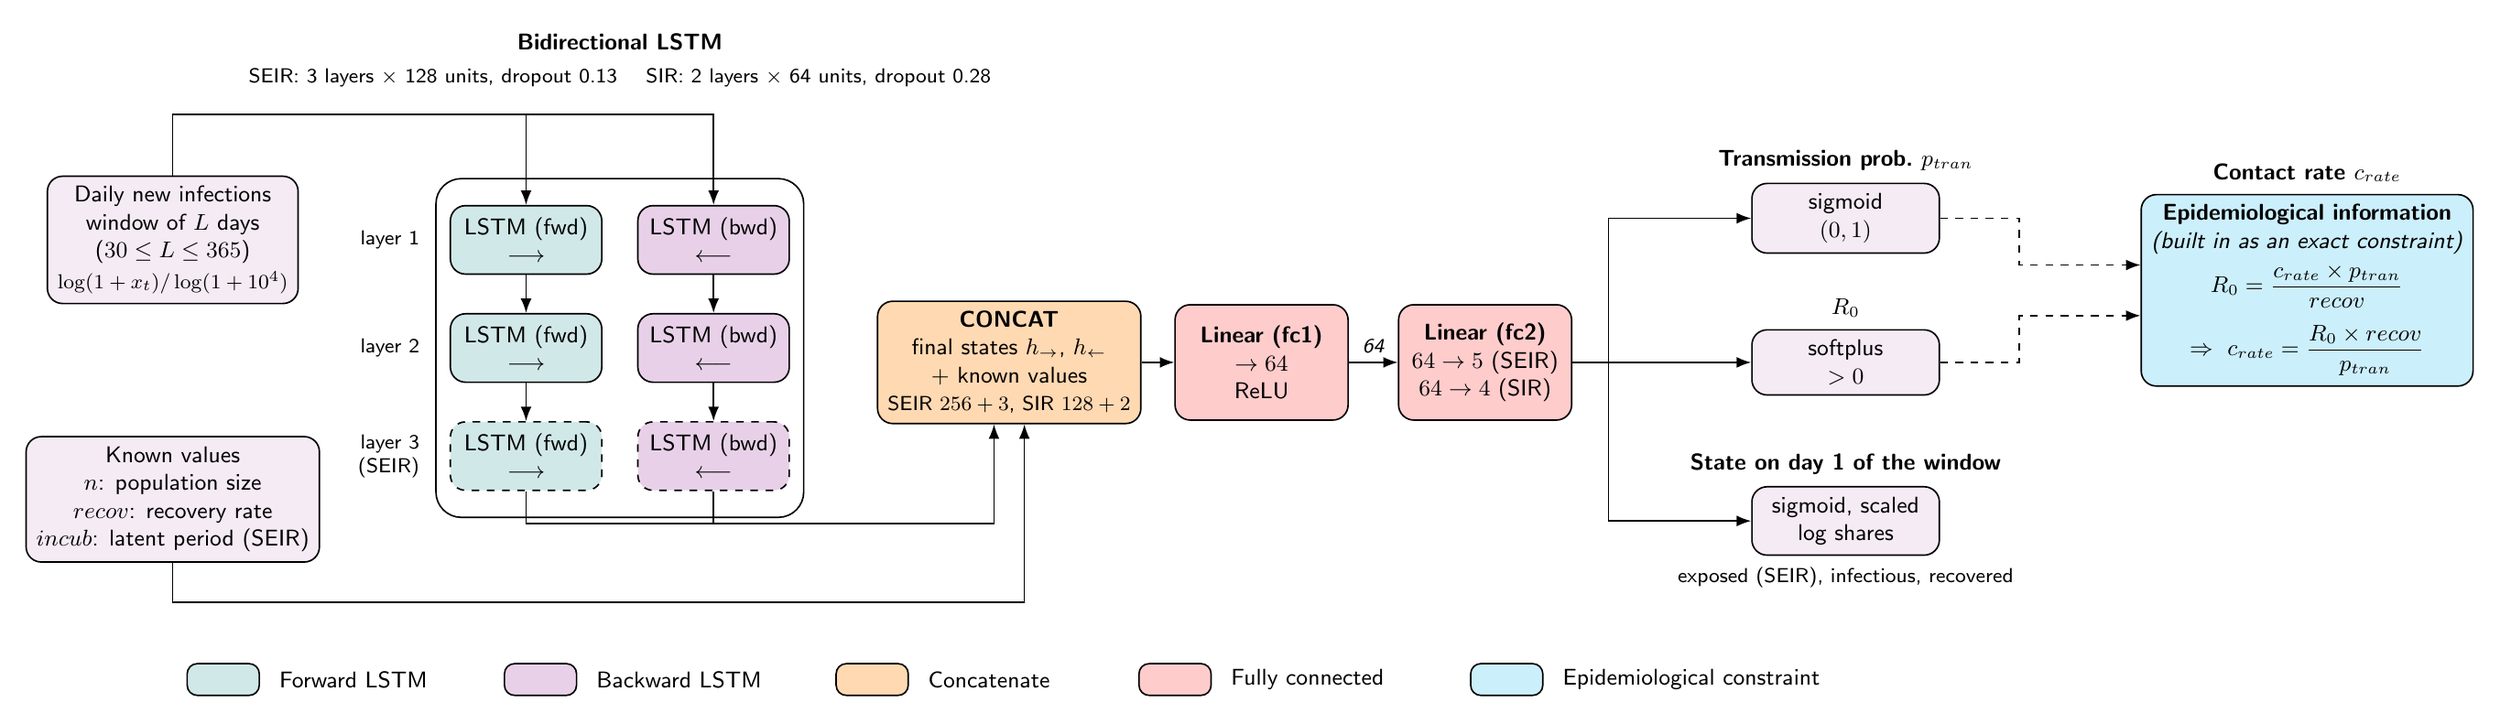
\begin{tikzpicture}[
  font=\sffamily\small, >=Latex, line width=0.6pt,
  box/.style={draw, rounded corners=6pt, align=center, inner sep=4pt},
  inp/.style={box, fill=violet!8, minimum width=3.2cm},
  fwd/.style={box, fill=teal!18, minimum width=2.1cm, minimum height=0.95cm},
  bwd/.style={box, fill=violet!18, minimum width=2.1cm, minimum height=0.95cm},
  catbox/.style={box, fill=orange!30, minimum width=3.6cm, minimum height=1.6cm},
  fcbox/.style={box, fill=red!20, minimum width=2.4cm, minimum height=1.6cm},
  outbox/.style={box, fill=violet!8, minimum width=2.6cm},
  der/.style={box, fill=cyan!20, minimum width=3.0cm},
  lab/.style={font=\sffamily\bfseries\small}
]
% Inputs
\node[inp] (inc) at (0, 2.6) {Daily new infections\\ window of $L$ days\\ ($30 \le L \le 365$)\\[1pt] {\footnotesize $\log(1+x_t)/\log(1+10^4)$}};
\node[inp] (known) at (0, -1.0) {Known values\\ $n$: population size\\ $recov$: recovery rate\\ $incub$: latent period (SEIR)};

% BiLSTM stack
\node[fwd] (f1) at (4.9, 2.6) {LSTM (fwd)\\ $\longrightarrow$};
\node[bwd] (b1) at (7.5, 2.6) {LSTM (bwd)\\ $\longleftarrow$};
\node[fwd] (f2) at (4.9, 1.1) {LSTM (fwd)\\ $\longrightarrow$};
\node[bwd] (b2) at (7.5, 1.1) {LSTM (bwd)\\ $\longleftarrow$};
\node[fwd, dashed] (f3) at (4.9, -0.4) {LSTM (fwd)\\ $\longrightarrow$};
\node[bwd, dashed] (b3) at (7.5, -0.4) {LSTM (bwd)\\ $\longleftarrow$};
\node[font=\sffamily\footnotesize, anchor=east] at (3.55, 2.6) {layer 1};
\node[font=\sffamily\footnotesize, anchor=east] at (3.55, 1.1) {layer 2};
\node[font=\sffamily\footnotesize, anchor=east, align=right] at (3.55, -0.4) {layer 3\\ (SEIR)};
\draw[rounded corners=10pt] (3.65, -1.25) rectangle (8.75, 3.45);
\node[lab, align=center] at (6.2, 5.35) {Bidirectional LSTM};
\node[font=\sffamily\footnotesize, align=center] at (6.2, 4.85) {SEIR: 3 layers $\times$ 128 units, dropout 0.13 \quad SIR: 2 layers $\times$ 64 units, dropout 0.28};
\foreach \a/\b in {f1/f2, f2/f3, b1/b2, b2/b3} \draw[->] (\a) -- (\b);

% Input routing (both directions read the whole window)
\draw[->] (inc.north) -- ++(0, 0.85) -| (f1.north);
\draw[->] (inc.north) ++(0, 0.85) -| (b1.north);

% Final states and known values to the concatenation
\node[catbox] (cat) at (11.6, 0.9) {\textbf{CONCAT}\\ final states $h_{\rightarrow}$, $h_{\leftarrow}$\\ + known values\\ {\footnotesize SEIR $256+3$, SIR $128+2$}};
\draw[->] (f3.south) -- ++(0, -0.45) -| ([xshift=-6pt]cat.south);
\draw (b3.south) -- ++(0, -0.45);
\draw[->] (known.south) -- ++(0, -0.55) -| ([xshift=6pt]cat.south);

% Dense layers
\node[fcbox] (fc1) at (15.1, 0.9) {\textbf{Linear (fc1)}\\ $\to 64$\\ ReLU};
\node[fcbox] (fc2) at (18.2, 0.9) {\textbf{Linear (fc2)}\\ $64 \to 5$ (SEIR)\\ $64 \to 4$ (SIR)};
\draw[->] (cat) -- (fc1);
\draw[->] (fc1) -- node[above, font=\sffamily\footnotesize\itshape] {64} (fc2);

% Outputs
\node[outbox] (o1) at (23.2, 2.9) {sigmoid\\ $(0,1)$};
\node[lab, above=1pt of o1] {Transmission prob.\ $p_{tran}$};
\node[outbox] (o2) at (23.2, 0.9) {softplus\\ $>0$};
\node[lab, above=1pt of o2] {$R_0$};
\node[outbox] (o3) at (23.2, -1.3) {sigmoid, scaled\\ log shares};
\node[lab, above=1pt of o3, align=center] {State on day 1 of the window};
\node[font=\sffamily\footnotesize, below=1pt of o3, align=center] {exposed (SEIR), infectious, recovered};
\draw (fc2.east) -- ++(0.5, 0) coordinate (split);
\foreach \o in {o1, o2, o3} \draw[->] (split) |- (\o.west);

% Derived quantity
\node[der] (crate) at (29.6, 1.9) {\textbf{Epidemiological information}\\ \textit{(built in as an exact constraint)}\\[3pt]
  $R_0 = \dfrac{c_{rate} \times p_{tran}}{recov}$\\[6pt] $\Rightarrow\ c_{rate} = \dfrac{R_0 \times recov}{p_{tran}}$};
\node[lab, above=1pt of crate] {Contact rate $c_{rate}$};
\draw[->, dashed] (o1.east) -- ++(1.1, 0) |- ([yshift=10pt]crate.west);
\draw[->, dashed] (o2.east) -- ++(1.1, 0) |- ([yshift=-10pt]crate.west);

% Legend
\begin{scope}[shift={(0.2, -3.5)}, every node/.style={font=\sffamily\small}]
  \foreach \c/\t/\x in {teal!18/Forward LSTM/0, violet!18/Backward LSTM/4.4, orange!30/Concatenate/9.0,
                        red!20/Fully connected/13.2, cyan!20/Epidemiological constraint/17.8} {
    \draw[rounded corners=4pt, fill=\c] (\x, -0.22) rectangle ++(1.0, 0.44);
    \node[anchor=west] at (\x + 1.15, 0) {\t};
  }
\end{scope}
\end{tikzpicture}
}
\caption{The DeepIMC network. A bidirectional LSTM reads the window of daily new infections forwards and
backwards; its final states are joined with the known values and passed through two dense layers, which
give the transmission probability, $R_0$ and the state of the epidemic on the first day of the window. The
epidemiological relation $R_0 = c_{rate}\,p_{tran}/recov$ is built in as an exact constraint: the contact
rate is computed from $R_0$ and $p_{tran}$, so the three parameters always agree. The shipped models average five such networks, trained with
different random seeds, and attach a 95\% range to $R_0$ from 500 similar calibration windows
(Section~\ref{sec:range}).}
\label{fig:architecture}
\end{figure}

\paragraph{Outputs.} The network predicts $p_{tran}$, $R_0$ and the logarithm of each state share on
the first day of the window. The contact rate is then computed from (\ref{eq:R0}) as $c_{rate} = R_0
\, p_{recov}/p_{tran}$, so the three parameters always agree with each other.

\paragraph{Epidemiological information.} A network that predicts $p_{tran}$, $c_{rate}$ and $R_0$ as three
separate outputs can return values that contradict (\ref{eq:R0}); a common remedy is to add a penalty such
as $\big(R_0\,p_{recov} - p_{tran}\,c_{rate}\big)^2$ to the loss, which pushes the outputs towards agreement
without guaranteeing it. DeepIMC builds this relation into the network instead: because $c_{rate}$ is
computed from $R_0$ and $p_{tran}$, the relation holds exactly for every window, which is equivalent to a
penalty with infinite weight. The penalty term is then always zero and is not needed in the loss.

\paragraph{Training.} The network was trained to minimize the mean squared error of the scaled
targets, with the Adam optimizer \autocite{kingma2015adam}, batches of 32 windows, and a learning rate
that starts at $7.2 \times 10^{-4}$ (SEIR) or $7.9 \times 10^{-4}$ (SIR) and decreases along a cosine
curve to 1\% of that value over 50 epochs \autocite{loshchilov2017sgdr}. Twenty percent of the
epidemics were held out for validation, and the weights of the epoch with the lowest validation
error were kept. We trained five networks with different random seeds and average their outputs.

\paragraph{Hyperparameter search.} The learning rate, batch size, number of layers, number of units and
dropout were chosen with Optuna \autocite{akiba2019optuna}, in 40 trials of 20 epochs on 100,000 of
the training epidemics (Appendix~\ref{app:training}).

\subsection{Uncertainty in $R_0$}\label{sec:range}

A single pass of the network gives point estimates. To attach a range to $R_0$, we simulated 100,000
further epidemics, cut one random window from each, and recorded DeepIMC's error on each of these
\emph{calibration windows}. For a new window, we find the 500 calibration windows that are most
similar to it---with similar estimates of $R_0$ and of the starting state, similar known values and a
similar length---and use the spread of their errors. The 2.5\% and 97.5\% quantiles of those errors,
added to the estimate, give the 95\% range of $R_0$. The same 500 errors, in $R_0$ and in the state
shares, give 500 plausible parameter sets, which are used to simulate the epidemic forward.

\subsection{From estimates to epidemic curves}\label{sec:prediction}

\paragraph{Model simulation.} To see what an estimate implies for the epidemic, we run the agent-based
model 500 times from the estimated state on the first day of the window, each run with parameters drawn
from the method's uncertainty: DeepIMC's 500 parameter sets, the ABC methods' posterior samples, or
the single estimate of differential evolution and Nelder--Mead. For every day, the 2.5\%, 50\% and
97.5\% quantiles of the runs give the regenerated curve (the median) and its 95\% band, both in the
window and for the following days.

\paragraph{The renewal equation.} A much faster alternative is the renewal equation
\autocite{fraser2007estimating,wallinga2007generation}, which gives the expected number of new
infectious people on day $t$ as
\begin{equation}\label{eq:renewal}
C_t = R_0\,\frac{S_{t-1}}{N}\sum_{k\ge 1} g_k\, C_{t-k},
\end{equation}
where $S_t$ is the number susceptible and $g_k$ the generation interval of the model, the probability
that a transmission happens $k$ days after the infector was infected. Because the latent and
infectious periods of our models are geometric, the sum can be carried forward day by day
(Appendix~\ref{app:renewal}). The renewal equation gives the model's average curve; we add Poisson
noise around it to obtain a band. We start it either from DeepIMC's estimated state (renewal A) or
from a state that the renewal equation itself fits to the window by least squares, with $R_0$ fixed
at 30 values from DeepIMC's range (renewal B). The main results use the agent-based model; the renewal equation is
evaluated as a faster alternative in the supplement (Appendix~\ref{sec:res-renewal}).

\subsection{Comparison methods}\label{sec:baselines}

We compared DeepIMC with four standard calibration methods, set up as a practitioner with basic
knowledge of them would use them: established implementations, their default settings, and only
the changes needed for them to work with these models (Table~\ref{tab:baselines},
Appendix~\ref{app:baselines}). Using default settings is deliberate: one of DeepIMC's aims is to
spare the user these choices, so the comparison shows what a user obtains without tuning.

\paragraph{The same problem for every method.} All methods receive the same window and known values
and search the same unknowns within the same ranges as DeepIMC: $R_0$ between 0.8 and 5, and the
state on the first day of the window (the shares exposed, infectious and recovered, searched on the
logarithmic scale between $10^{-4}$ and 0.4, or 0.95 for the recovered share). Because the curve
reveals $R_0$ but not the split into $p_{tran}$ and $c_{rate}$ (Section~\ref{sec:models}), the
comparison methods fix $c_{rate}$ at the middle of its range and obtain $p_{tran}$ from (\ref{eq:R0}).

\paragraph{Comparing a simulated curve with the data.} Following common practice in approximate
Bayesian computation \autocite{beaumont2002approximate}, ABC-MCMC and ABC-SMC compare \emph{summary
statistics} of the observed and simulated curves: the mean, the peak and the minimum of the daily
counts, the day of the peak, the means of the first and the last week, the days by which 25\%, 50\%
and 75\% of the window's cases had occurred, and the growth rates over the first and the last two
weeks (Appendix~\ref{app:baselines}). Each statistic is divided by its spread over simulations from
the prior, so that statistics measured in different units count equally
\autocite{prangle2017adapting}. Differential evolution and Nelder--Mead minimize the sum of squared
differences between the observed counts and the simulated daily new infections, using one model run
with a fixed random seed per candidate so that the same candidate always receives the same fit.
Appendix~\ref{app:abc-sensitivity} compares the ABC methods on summary statistics with the same
methods on the whole curve.

\begin{table}[htbp]
\centering
\caption{The comparison methods and their settings. All are run with their default settings, except
the two limits of ABC-SMC (see text).}
\label{tab:baselines}
\small
\begin{tabular}{>{\raggedright\arraybackslash}p{2.3cm} >{\raggedright\arraybackslash}p{7.0cm} >{\raggedleft\arraybackslash}p{1.9cm} >{\raggedright\arraybackslash}p{3.1cm}}
\toprule
Method & Settings & Model runs per window & Stopping rule \\
\midrule
DeepIMC & average of 5 networks; $R_0$ range from 500 similar calibration windows & 0 & one pass of the networks \\
ABC-MCMC \autocite{marjoramMarkovChainMonte2003} & \texttt{epiworldRcalibrate}: summary statistics; 3,000 random-walk steps (1,500 burn-in), proposal s.d.\ 8\% of each range, Gaussian kernel with the tolerance set from 200 prior simulations & about 3,200 & after 3,000 steps \\
ABC-SMC \autocite{toniApproximateBayesianComputation2008} & \texttt{epiworldRcalibrate}: summary statistics; 200 particles, 6 generations, each tolerance the median distance of the previous generation; at most 30,000 model runs and 20,000 attempts per generation & up to 30,000 & after 6 generations \\
DE \autocite{storn1997differential} & \texttt{DEoptim} \autocite{mullen2011deoptim}: population of 10 times the number of unknowns, 200 generations, $F = 0.8$, $CR = 0.5$; sum of squared differences & 6,030--8,040 & after 200 generations \\
Nelder--Mead \autocite{nelder1965simplex} & \texttt{stats::optim}: started at the middle of the ranges, values outside the ranges rejected; sum of squared differences & about 100 & relative change of the fit below $1.5\times10^{-8}$, or 500 runs \\
\bottomrule
\end{tabular}
\end{table}

\paragraph{Necessary adjustments.} With its default limits of 8,000 model runs and 5,000 attempts per
generation, ABC-SMC stopped before finishing on most simulated SEIR windows; we raised the two limits,
as its error message suggests. Differential evolution always runs its 200 generations, because its
default early-stopping rule (no improvement for 200 generations) cannot be met within 200 generations.

\subsection{Evaluation on simulated data}\label{sec:eval-sim}

Simulated data are the only setting in which the true parameters and the true epidemic are known, so
most of the evaluation uses them. All test epidemics were simulated with the distributions of
Table~\ref{tab:priors} but with new random seeds, and none was used in training.

\paragraph{DeepIMC alone, by window length.} To show how DeepIMC's accuracy depends on how much data it
sees, we simulated 1,000 test epidemics per model and evaluated DeepIMC on windows of 30, 61, 90, 120,
180, 270 and 365 days starting at the beginning (day 1), the middle and the end (the last informative
day) of each epidemic that lasts that long.

\paragraph{All methods: 10,000 test windows.} For the comparison with the other methods, we simulated
10,000 further test epidemics (5,000 per model) and took one window from each: a random length between
30 and 180 days at a random start among the epidemic's informative days (epidemics with fewer than 30
informative days were skipped). We call a window \emph{early}, \emph{middle} or \emph{late} when it
starts in the first, second or last third of the possible starts. Every method calibrated every window.

\paragraph{Parameter recovery.} For each parameter we report the mean absolute error (MAE) over the
windows, $\frac1n\sum_i|\hat\theta_i-\theta_i|$, where $\theta_i$ is the true value and $\hat\theta_i$
the estimate, for $R_0$, $p_{tran}$ and $c_{rate}$. The starting-state error is the mean absolute error
of the state shares, in percentage points. For DeepIMC and the ABC methods, which give a 95\% range for
$R_0$, we also report how often the true value lies inside it; a well-calibrated range should contain it
about 95\% of the time.

\paragraph{Recovery of the epidemic curves.} A method can estimate parameters well and still reproduce
the epidemic poorly, or the reverse. We therefore used each method's estimates to regenerate the epidemic
(500 model runs, Section~\ref{sec:prediction}) for the window and the 14 days after it, and compared the
regenerated curves with the true curves of the test epidemic in three ways:
\begin{itemize}[leftmargin=*]
\item the daily new infections in the window, the data each method saw;
\item the number of people currently infectious in the window, which no method observes;
\item the daily new infections over the 14 days after the window, a short-term prediction.
\end{itemize}
For each, we report the coverage of the 95\% band and the MAE of the regenerated median curve
(Section~\ref{sec:scores}).

\subsection{Evaluation on real data}\label{sec:eval-real}

\paragraph{Choosing appropriate datasets.} Real data have no true parameter values, so on real data the
methods are compared by how well the curves regenerated from their estimates match the observed counts.
For this comparison to be meaningful, the data should measure what the models describe: the daily
number of new infections. We therefore examined what each candidate dataset counts. Case counts by date
of test report follow testing and reporting as much as infection: in the Utah COVID-19 cases, for
example, Sundays are 30--40\% below the weekly average, and after home testing became common most
infections were not reported \autocite{utahdhhs2025covid}. Counts by date of symptom onset, and hospital
admissions by date of admission, follow new infections more closely: they are not shaped by the
reporting week, and a stable fraction of infections leads to them after a fairly constant delay. We
selected five such datasets (Table~\ref{tab:datasets}), covering four diseases, and kept the Utah
COVID-19 cases by test report date as a contrast.

\begin{table}[htbp]
\centering
\caption{The real datasets: what each counts, its source, and the known values used for each disease
(SEIR latent period incub in days and recovery rate; SIR recovery rate).}
\label{tab:datasets}
\small
\begin{tabular}{>{\raggedright\arraybackslash}p{2.6cm} >{\raggedright\arraybackslash}p{3.6cm} >{\raggedright\arraybackslash}p{3.0cm} >{\raggedleft\arraybackslash}p{1.2cm} >{\raggedright\arraybackslash}p{3.4cm}}
\toprule
Dataset & What is counted (by date of) & Period and source & Windows per model & Known values (SEIR; SIR) \\
\midrule
Utah COVID-19 & confirmed COVID-19 hospital admissions (admission) & three waves, Sep 2020--Mar 2022; Utah DHHS \autocite{utahdhhs2025covid} & 27 & incub 5.2, $p_{recov}$ 0.25; $p_{recov}$ 0.133 \autocite{li2020early} \\
Utah influenza & confirmed influenza hospital admissions (admission) & 2022--23 and 2023--24 seasons; US HHS \autocite{hhs2024hospital} & 18 & incub 1.4, $p_{recov}$ 0.25; $p_{recov}$ 0.25 \autocite{lessler2009incubation,cori2013new} \\
Baltimore influenza 1918 & influenza cases from a house-to-house survey (symptom onset) & 92 days, autumn 1918 \autocite{frost1919influenza,cori2013new} & 9 & as Utah influenza \\
Hong Kong SARS 2003 & SARS cases (symptom onset) & 107 days, 2003 \autocite{cori2009temporal} & 9 & incub 6.4, $p_{recov}$ 0.25; $p_{recov}$ 0.119 \autocite{donnelly2003epidemiological,lipsitch2003transmission} \\
Sierra Leone Ebola 2014--15 & confirmed and suspected cases (symptom onset) & May 2014--Sep 2015 \autocite{fang2016ebola} & 9 & incub 11.4, $p_{recov}$ 0.25; $p_{recov}$ 0.071 \autocite{who2014ebola} \\
\midrule
\textit{Contrast:} Utah COVID-19 cases & confirmed cases (test report) & as Utah COVID-19 & 27 & as Utah COVID-19 \\
\bottomrule
\end{tabular}
\end{table}

\paragraph{Known values.} The known values for each disease come from published estimates of the mean
incubation period and the mean serial interval (the time between the symptom onsets of an infector and
the person they infect). In the SEIR model, the latent period is set to the incubation period, and the
infectious period to the serial interval minus the incubation period, but at least 4 days, the shortest
in the training data. In the SIR model, which has no latent period, the infectious period is set to the
serial interval, within the trained range of 4 to 14 days.

\paragraph{Population size.} The models describe an epidemic in which every new infection is counted, in
a population of 5,000 to 10,000. Real counts cover only a fraction of infections in a much larger
population, and the reported fraction and the population size cannot be separated from a curve alone.
We therefore read every dataset as the complete incidence of an effective population of $N = 10{,}000$.
The Utah COVID-19 cases are far more than 10,000 people could produce and were scaled to cases per
10,000 residents.

\paragraph{Windows.} In each wave or epidemic we took windows of 30, 60 and 90 days at the beginning, the
middle (centred on the peak of the 7-day average) and the end, and scored the bands on the window and on
the next 14 days where the data continue.

\subsection{Scores}\label{sec:scores}

A 95\% band $[l_t, u_t]$ and its median curve $m_t$ are compared with the values $y_t$ (true or
observed) over $T$ days by two scores.
\begin{itemize}[leftmargin=*]
\item \emph{Coverage}, the percentage of days on which the value lies inside the band,
$\frac{100}{T}\sum_t \mathbf{1}(l_t\le y_t\le u_t)$. About 95\% is ideal for a 95\% band; much lower
means the band misses the data, and 100\% can mean the band is too wide.
\item \emph{Mean absolute error} (MAE) of the median curve, $\frac1T\sum_t |m_t-y_t|$, in daily counts
(or, for the number currently infectious, in people). Lower is better.
\end{itemize}
The two scores answer different questions. Coverage asks whether the band is honest about its
uncertainty; the MAE asks how close the method's best guess is to the truth. A method can reach high
coverage with very wide bands while its median curve is far from the data, so we always report both.
For the same reason we report, besides the coverage of the $R_0$ ranges, their average width.

\subsection{Computing time}\label{sec:eval-time}

All timings were made on CPUs only, without a GPU, so that the methods are compared on the same
hardware. Every method ran on one CPU core of the same computer (an AMD EPYC 7601 processor), on 20
windows of 30 to 180 days (10 per model) from the simulated test set. For DeepIMC we measured its first
call in a new R session, through the package's functions (which start Python and load the networks), one
window at a time, and many windows in one pass. We also measured
the cost of turning a fit into a 95\% band. Training DeepIMC is a separate, one-time cost: we report the
CPU time to simulate the training epidemics and the time to train one network, on CPUs (estimated from
one training epoch) and on the GPUs we actually used.

% =============================================================================
\section{Results}\label{sec:results}

\subsection{How DeepIMC's accuracy depends on the window}\label{sec:res-bilstm}

The first question is how much data DeepIMC needs. Table~\ref{tab:bilstm-length} shows its errors on
windows of increasing length that start at the beginning of the test epidemics.

The error in $R_0$ falls quickly as the window grows. With 30 days of data the mean absolute error is
0.28 for the SEIR model and 0.14 for the SIR model; with 180 days it is 0.06 and 0.05. The SEIR model
needs more data than the SIR model, because the latent period delays the effect of transmission on the
curve. Windows that start in the middle or at the end of an epidemic are harder than those that start at
the beginning, most of all when they are short (column ``any position''): in these windows part of the
population is already immune, and the network must also work out how many people have been infected
before the window begins.

Figure~\ref{fig:deepimc-by-window} shows the same results by position. The error is largest for short
windows at the end of an epidemic (0.76 for 30-day SEIR windows), where little of the epidemic is left to
see; it falls below 0.2 once the window is 120 days long, and for windows of 270 days or more the position no
longer matters. The coverage of the true curves stays above 94\% for every length and position, except for
the true number of infectious people in 30-day SEIR windows at the beginning of an epidemic (90\%).

The 95\% range of $R_0$ contained the true value in 88--99\% of the SEIR windows and 92--100\% of the SIR
windows, depending on the length; over all windows, 94\% for both models. The range is slightly too
narrow for the shortest SEIR windows and well calibrated otherwise.

\begin{table}[htbp]
\centering
\caption{DeepIMC on simulated windows that start at the beginning of the test epidemics, by window
length. MAE of $R_0$ for these windows and for windows at any position (beginning, middle and end);
percentage of windows whose 95\% range contains the true $R_0$; MAE of $p_{tran}$ and $c_{rate}$, with
in brackets the error of a guess that knows $R_0$ exactly but not how it splits into $p_{tran}$ and
$c_{rate}$; coverage of the true daily new infections and of the true number currently infectious by
the 95\% band of 100 simulations from the estimates, over windows at any position (100 test epidemics per
length and position).}
\label{tab:bilstm-length}
\small
\resizebox{\textwidth}{!}{%
\begin{tabular}{llrrrrrrrr}
\toprule
& Window & & \multicolumn{2}{c}{$R_0$ MAE} & True $R_0$ & $p_{tran}$ MAE & $c_{rate}$ MAE & \multicolumn{2}{c}{Coverage (\%)} \\
\cmidrule(lr){4-5}\cmidrule(lr){9-10}
Model & (days) & Windows & beginning & any position & in range (\%) & (guess) & (guess) & new inf. & infectious \\
\midrule
SEIR & 30  & 990 & 0.284 & 0.438 & 87.7 & 0.0157 (0.0147) & 2.60 (2.56) & 96.9 & 94.1 \\
     & 61  & 960 & 0.107 & 0.222 & 94.7 & 0.0145 (0.0144) & 2.59 (2.56) & 97.5 & 97.8 \\
     & 90  & 883 & 0.087 & 0.161 & 95.7 & 0.0139 (0.0138) & 2.59 (2.55) & 97.4 & 98.2 \\
     & 120 & 746 & 0.078 & 0.126 & 96.5 & 0.0131 (0.0130) & 2.55 (2.52) & 97.4 & 98.6 \\
     & 180 & 475 & 0.063 & 0.092 & 95.2 & 0.0109 (0.0108) & 2.47 (2.47) & 97.5 & 98.7 \\
     & 270 & 178 & 0.048 & 0.052 & 97.1 & 0.0075 (0.0074) & 2.38 (2.37) & 97.3 & 98.5 \\
     & 365 & 80  & 0.041 & 0.041 & 98.9 & 0.0073 (0.0071) & 2.65 (2.57) & 96.8 & 97.4 \\
\midrule
SIR  & 30  & 982 & 0.135 & 0.260 & 93.6 & 0.0643 (0.0685) & 1.01 (0.97) & 98.4 & 98.5 \\
     & 61  & 572 & 0.098 & 0.145 & 94.6 & 0.0486 (0.0482) & 1.07 (1.00) & 98.5 & 98.7 \\
     & 90  & 293 & 0.088 & 0.119 & 95.0 & 0.0364 (0.0356) & 1.09 (1.02) & 98.6 & 99.3 \\
     & 120 & 159 & 0.075 & 0.098 & 93.9 & 0.0329 (0.0319) & 1.14 (1.04) & 98.6 & 99.3 \\
     & 180 & 53  & 0.052 & 0.067 & 91.8 & 0.0280 (0.0280) & 1.14 (1.08) & 98.0 & 99.0 \\
     & 270 & 18  & 0.037 & 0.042 & 95.2 & 0.0239 (0.0242) & 0.99 (1.02) & 97.7 & 98.7 \\
     & 365 & 8   & 0.029 & 0.029 & 100.0 & 0.0153 (0.0150) & 0.91 (0.83) & 96.1 & 95.4 \\
\bottomrule
\end{tabular}}
\end{table}

\begin{figure}[htbp]
\centering
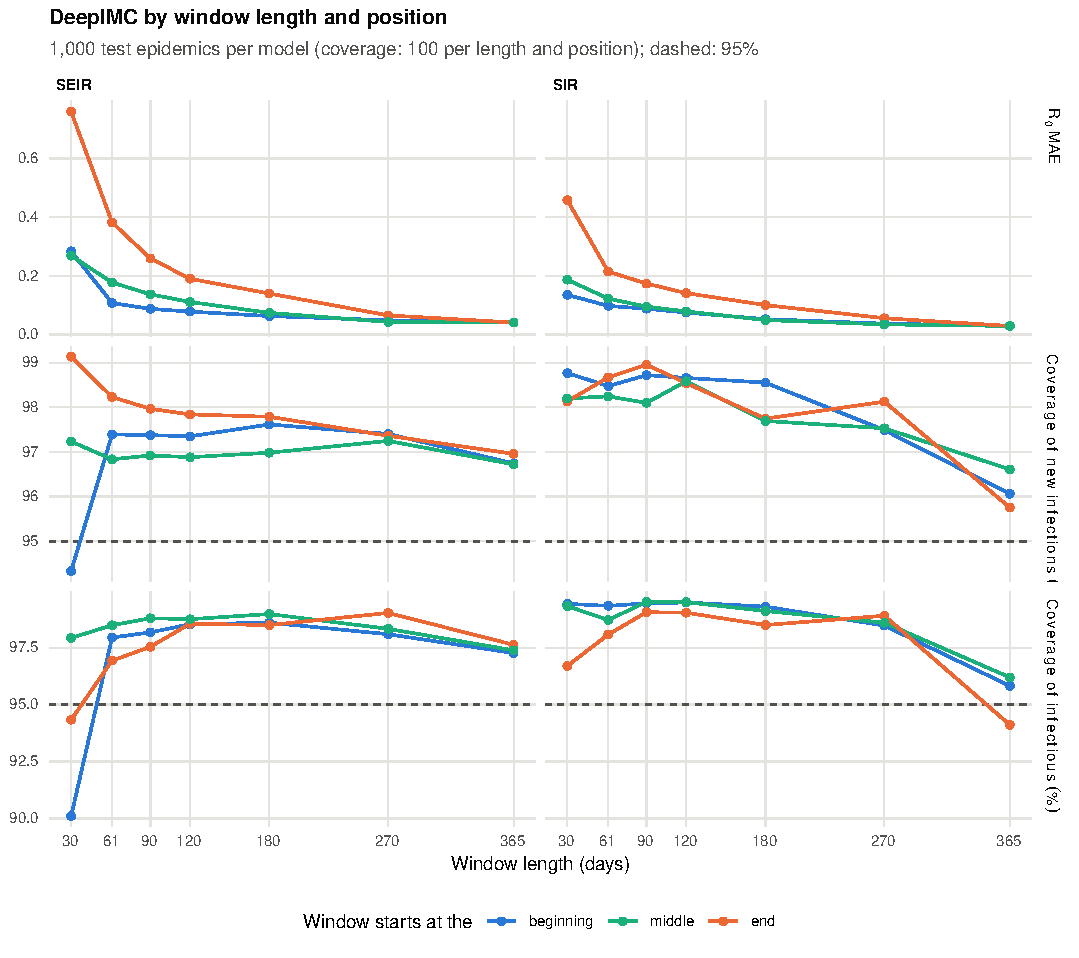
\includegraphics[width=\textwidth]{figures/deepimc_by_window.pdf}
\caption{DeepIMC by window length and position: $R_0$ mean absolute error, and coverage of the true daily
new infections and of the true number currently infectious by the 95\% band, for windows that start at the
beginning, the middle and the end of the test epidemics.}
\label{fig:deepimc-by-window}
\end{figure}

\paragraph{The transmission probability and the contact rate.} The errors in $p_{tran}$ and $c_{rate}$
behave differently from the error in $R_0$: they hardly change with the window length, and they are
almost exactly those of the guess that knows $R_0$ and picks a typical split
(Table~\ref{tab:bilstm-length}). For 61-day SEIR windows, for example, DeepIMC's $p_{tran}$ error is
0.0145 against 0.0144 for the guess, and its $c_{rate}$ error 2.59 against 2.56. This is what
Section~\ref{sec:models} predicts: the curve contains information about $R_0$, the product of the two,
but none about how it splits. No calibration method can do better from case curves alone.

\paragraph{The epidemic behind the window.} When the model is run forward from DeepIMC's estimates, the
true daily new infections fall inside the 95\% band on 96--99\% of the days at every window length, and
the true number of infectious people---which the network never sees---on 94--99\% of the days. DeepIMC
therefore recovers not only $R_0$ but also the hidden state of the epidemic.

\subsection{Parameter recovery compared with standard methods}\label{sec:res-sim-params}

We now turn to the comparison with the four standard methods on the 10,000 simulated test windows. The
first question is how accurately each method recovers the parameters and the starting state.

\paragraph{$R_0$.} DeepIMC estimated $R_0$ with a mean absolute error of 0.17 in the SEIR windows and
0.14 in the SIR windows (Table~\ref{tab:sim-parameters}). The best comparison method was ABC-SMC for
SEIR (0.55) and differential evolution for SIR (0.36), so DeepIMC's error was about three times smaller
for SEIR and 2.6 times smaller for SIR. ABC-MCMC (0.81 for both models) and Nelder--Mead (0.95 and 0.65)
were the least accurate. On the same windows, every comparison method had a larger error than DeepIMC,
for every position of the window, and none of the 95\% bootstrap intervals of the paired differences
includes zero (Table~\ref{tab:sim-paired}). DeepIMC was more accurate than ABC-SMC on 82\% (SEIR) and
80\% (SIR) of the windows, and more accurate than differential evolution on 75\% and 72\%.

\paragraph{The position of the window.} Where the window comes from matters a great deal for the
comparison methods. On early windows, which contain the growth of the epidemic, differential evolution
came closest to DeepIMC (0.24 against 0.12 for SEIR, 0.17 against 0.11 for SIR). On middle and late
windows, where a method must also work out how many people were already infected or immune, the errors
of the comparison methods were two to four times larger than on early windows, while DeepIMC's errors
grew much less (to 0.16 and 0.25 for SEIR, 0.13 and 0.18 for SIR). Figure~\ref{fig:methods-by-window} breaks
these results down by window length as well: DeepIMC had the lowest $R_0$ error in every group of length and
position, and its advantage was largest for short windows in the middle and at the end of an epidemic, where
the comparison methods' errors were largest. Longer windows helped every method except ABC-MCMC, whose error
did not fall with the length of the window, and in SIR windows grew from 0.6--0.8 to 1.5--1.7. Figure~\ref{fig:parameter-recovery}
shows how the comparison methods fail: ABC-MCMC's estimates are pulled towards the middle of the range,
ABC-SMC underestimates many large values of $R_0$, and differential evolution and Nelder--Mead return
many estimates at the lower limit of 0.8 whatever the true value.

\paragraph{The range of $R_0$.} DeepIMC's 95\% range contained the true $R_0$ in 96\% of the windows for
both models, close to the nominal 95\%, with an average width of 0.90 (SEIR) and 0.70 (SIR). The ranges of
ABC-MCMC and ABC-SMC contained it about as often (96--98\%), but they were three to five times wider
(2.6 to 3.5, for a prior range of width 4.2): they were rarely wrong because they said little.

\paragraph{The transmission probability and the contact rate.} As expected from
Section~\ref{sec:models}, no method recovered $p_{tran}$ and $c_{rate}$ separately
(Figure~\ref{fig:parameter-recovery}, rows $p_{tran}$ and $c_{rate}$). DeepIMC's errors were close to
those of the guess that knows $R_0$ exactly and takes the middle of the range of the contact rate:
0.0147 against 0.0140 for $p_{tran}$ in SEIR windows, and 2.59 against 2.51 for $c_{rate}$. The comparison
methods fix $c_{rate}$ at the middle of its range, so their $c_{rate}$ error is that of the guess by
construction; their $p_{tran}$ errors are larger than DeepIMC's because their $R_0$ is less accurate.

\paragraph{The starting state.} The error of the estimated shares exposed, infectious and recovered at
the start of the window was 1.4 (SEIR) and 2.2 (SIR) percentage points for DeepIMC, against 4.1 to 9.7
and 4.5 to 10.0 for the comparison methods. ABC-SMC failed on 9 SEIR windows even with its raised limits;
they are left out of its averages.

\begin{table}[htbp]
\centering
\caption{Parameter recovery on the 10,000 simulated test windows (5,000 per model). MAE of $R_0$ for all
windows and for early, middle and late windows; for the methods that give a 95\% range of $R_0$, the
percentage of windows whose range contains the true value and the average width of the range; MAE of
$p_{tran}$ and $c_{rate}$, with the error of a guess that knows $R_0$ exactly and takes the middle of the
range of $c_{rate}$; starting-state error (percentage points). Bold: lowest error. The comparison methods
fix $c_{rate}$ at the middle of its range, so their $c_{rate}$ error is that of the guess.}
\label{tab:sim-parameters}
\small
\resizebox{\textwidth}{!}{\begin{tabular}{llrrrrrrrrr}
\toprule
 &  & \multicolumn{4}{c}{$R_0$ MAE} & \multicolumn{2}{c}{95\% range of $R_0$} & $p_{tran}$ & $c_{rate}$ & State \\
\cmidrule(lr){3-6}\cmidrule(lr){7-8}
Model & Method & all & early & middle & late & has true (\%) & width & MAE & MAE & error \\
\midrule
SEIR & DeepIMC & \textbf{0.17} & \textbf{0.12} & \textbf{0.16} & \textbf{0.25} & 95.9 & 0.90 & 0.0147 & 2.59 & \textbf{1.4} \\
 & ABC-MCMC & 0.81 & 0.69 & 0.82 & 0.93 & 95.6 & 3.55 & 0.0192 & 2.51 & 9.2 \\
 & ABC-SMC & 0.55 & 0.33 & 0.52 & 0.80 & 97.5 & 2.99 & 0.0170 & 2.51 & 4.9 \\
 & DE & 0.62 & 0.24 & 0.64 & 0.99 & -- & -- & 0.0187 & 2.51 & 4.1 \\
 & Nelder--Mead & 0.95 & 0.47 & 0.96 & 1.42 & -- & -- & 0.0223 & 2.51 & 9.7 \\
 & \textit{guess knowing $R_0$} &  &  &  &  &  &  & 0.0140 & 2.51 &  \\
\midrule
SIR & DeepIMC & \textbf{0.14} & \textbf{0.11} & \textbf{0.13} & \textbf{0.18} & 95.8 & 0.70 & 0.0685 & 1.05 & \textbf{2.2} \\
 & ABC-MCMC & 0.81 & 0.73 & 0.83 & 0.87 & 96.4 & 3.33 & 0.0810 & 1.01 & 10.0 \\
 & ABC-SMC & 0.40 & 0.27 & 0.34 & 0.57 & 98.4 & 2.57 & 0.0709 & 1.01 & 5.4 \\
 & DE & 0.36 & 0.17 & 0.39 & 0.54 & -- & -- & 0.0714 & 1.01 & 4.5 \\
 & Nelder--Mead & 0.65 & 0.24 & 0.68 & 1.05 & -- & -- & 0.0807 & 1.01 & 8.2 \\
 & \textit{guess knowing $R_0$} &  &  &  &  &  &  & 0.0716 & 1.01 &  \\
\bottomrule
\end{tabular}
}
\end{table}

\begin{table}[htbp]
\centering
\caption{Paired difference in the $R_0$ absolute error, comparison method minus DeepIMC, on the same
windows (positive: DeepIMC is more accurate), with 95\% bootstrap intervals.}
\label{tab:sim-paired}
\small
\resizebox{\textwidth}{!}{\begin{tabular}{llllll}
\toprule
Model & Method & All windows & Early & Middle & Late \\
\midrule
SEIR & ABC-MCMC & 0.64 (0.62, 0.65) & 0.57 (0.54, 0.59) & 0.66 (0.63, 0.69) & 0.69 (0.65, 0.72) \\
 & ABC-SMC & 0.38 (0.36, 0.39) & 0.21 (0.20, 0.23) & 0.36 (0.34, 0.39) & 0.56 (0.52, 0.59) \\
 & DE & 0.45 (0.43, 0.47) & 0.12 (0.11, 0.14) & 0.48 (0.45, 0.52) & 0.74 (0.70, 0.79) \\
 & Nelder--Mead & 0.77 (0.75, 0.80) & 0.36 (0.33, 0.38) & 0.80 (0.76, 0.85) & 1.18 (1.12, 1.23) \\
\midrule
SIR & ABC-MCMC & 0.67 (0.65, 0.68) & 0.62 (0.60, 0.65) & 0.70 (0.67, 0.73) & 0.69 (0.66, 0.72) \\
 & ABC-SMC & 0.25 (0.24, 0.27) & 0.16 (0.15, 0.17) & 0.21 (0.19, 0.23) & 0.39 (0.36, 0.42) \\
 & DE & 0.22 (0.20, 0.23) & 0.06 (0.04, 0.07) & 0.26 (0.24, 0.28) & 0.35 (0.33, 0.38) \\
 & Nelder--Mead & 0.51 (0.48, 0.53) & 0.13 (0.11, 0.14) & 0.55 (0.50, 0.59) & 0.87 (0.82, 0.92) \\
\bottomrule
\end{tabular}
}
\end{table}

\begin{figure}[htbp]
\centering
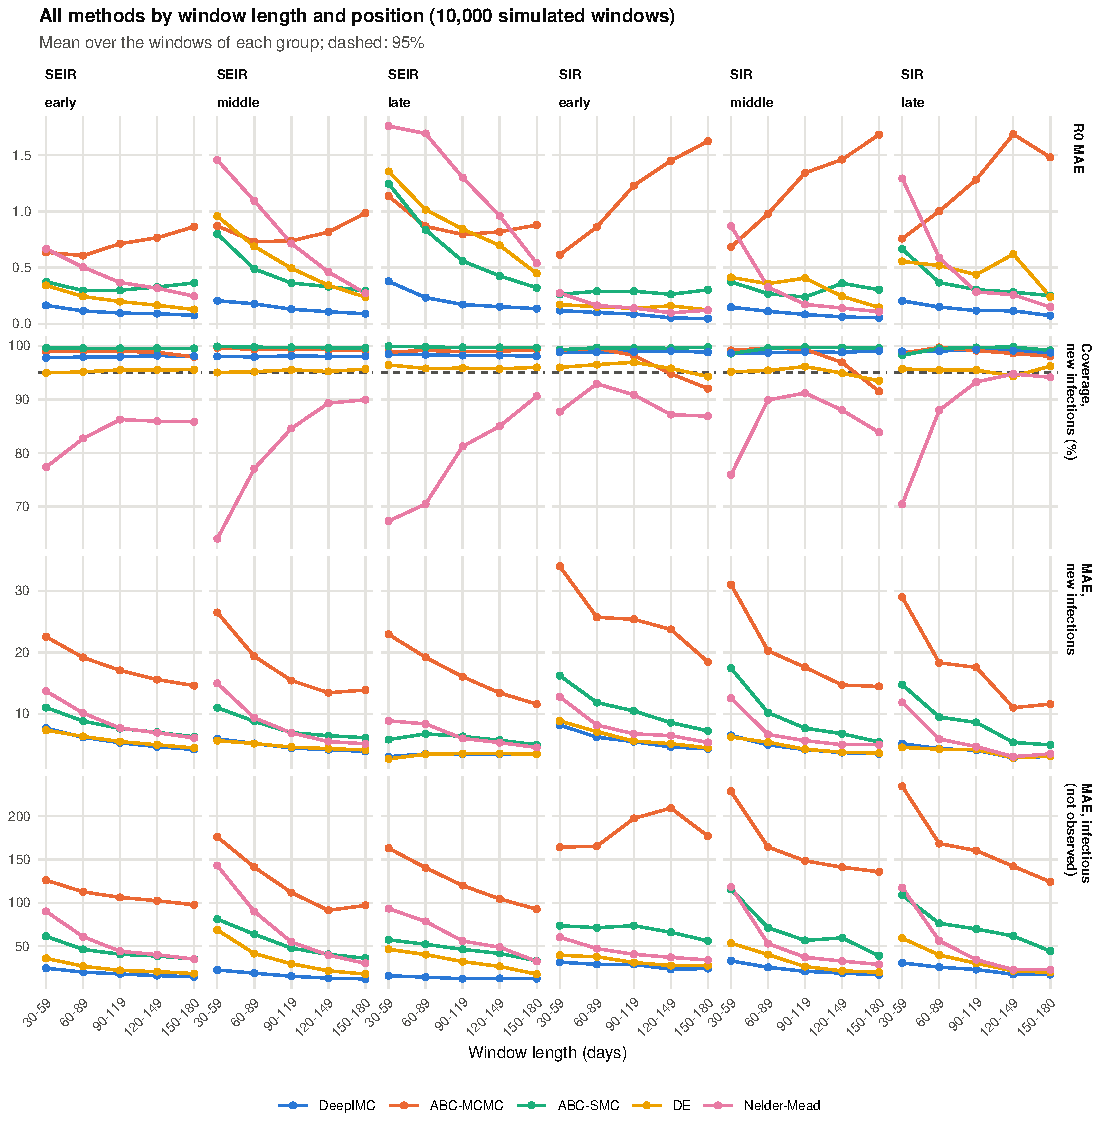
\includegraphics[width=\textwidth]{figures/methods_by_window_simulated.pdf}
\caption{All methods on the 10,000 simulated test windows, by window length (groups of 30 days) and position
(early, middle, late): $R_0$ mean absolute error; coverage of the true daily new infections in the window by
the 95\% band; MAE of the regenerated daily new infections in the window; and MAE of the regenerated number
currently infectious (not observed by any method). Dashed line: 95\%.}
\label{fig:methods-by-window}
\end{figure}

\begin{figure}[htbp]
\centering
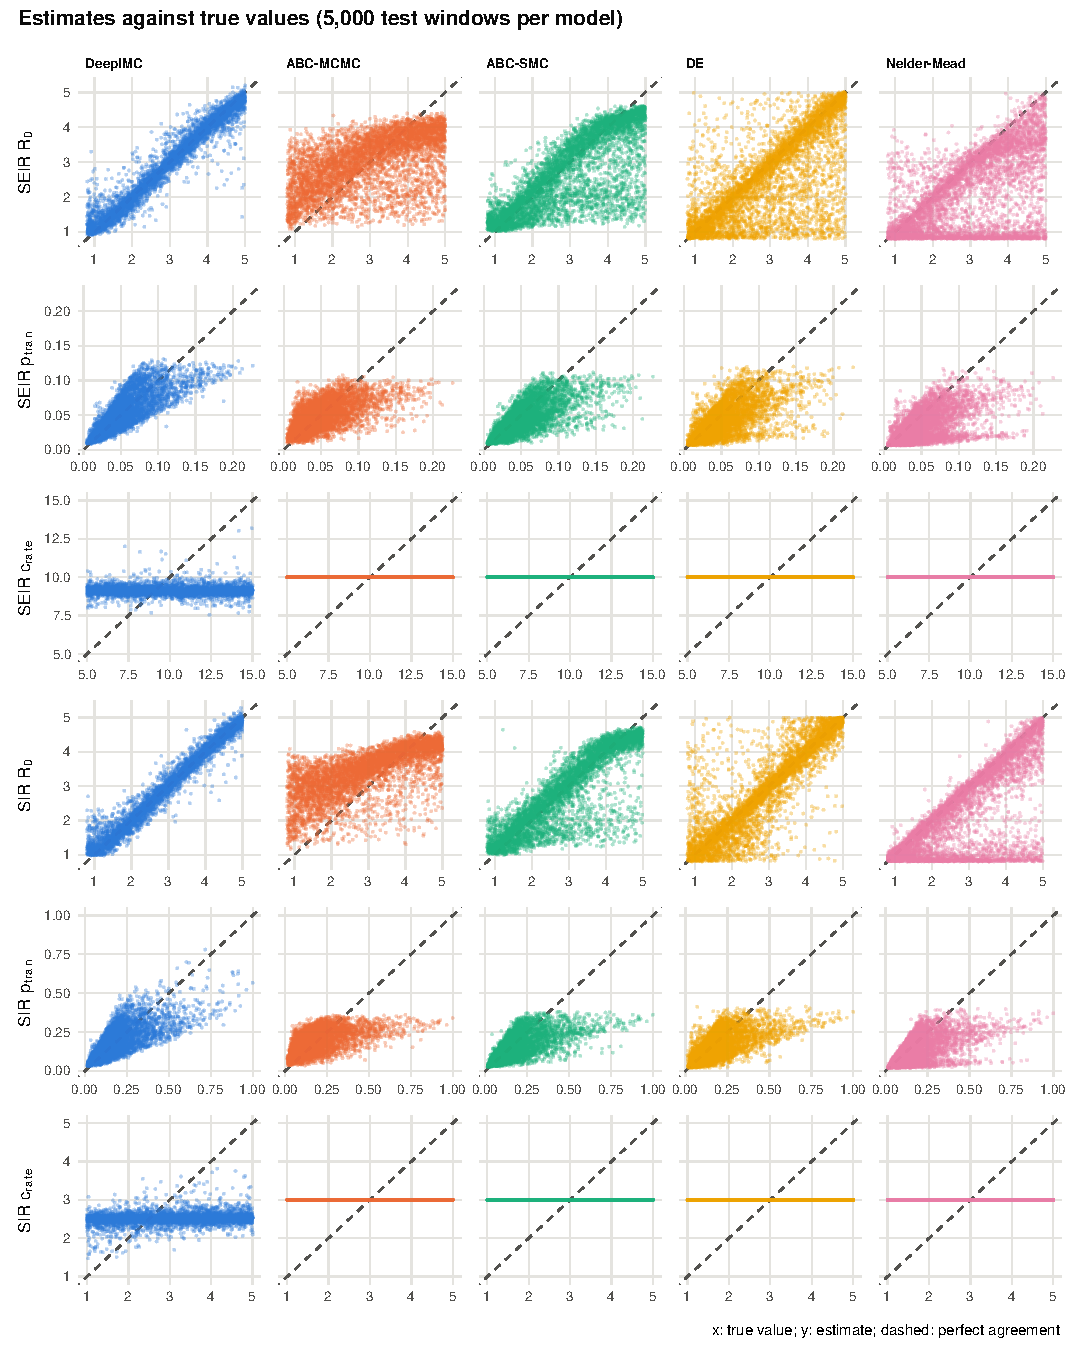
\includegraphics[width=\textwidth]{figures/parameter_recovery.pdf}
\caption{Estimated against true values of $R_0$, $p_{tran}$ and $c_{rate}$ for every simulated test
window and method; the dashed line is perfect agreement. DeepIMC's flat cloud for $c_{rate}$ shows that the
curve does not reveal it; the comparison methods fix it at the middle of its range.}
\label{fig:parameter-recovery}
\end{figure}

\subsection{Recovery of the epidemic curves}\label{sec:res-sim-curves}

The second question is whether each method's estimates reproduce the epidemic itself.

For each window, we ran the agent-based model 500 times from each method's estimates and compared the
regenerated curves with the true curves of the test epidemic (Table~\ref{tab:sim-curves},
Figures~\ref{fig:heatmap-sim}--\ref{fig:ridgelines}).

\paragraph{New infections in the window.} All methods except Nelder--Mead reproduced the curve they had
seen. The MAE of the regenerated median curve was 4.8 daily new infections for both DeepIMC and
differential evolution in the SEIR windows (6.1 and 6.2 in the SIR windows), against 7.8 to 18.8 for the
ABC methods (14.1 to 28.2) and 8.9 for Nelder--Mead (10.6). Differential evolution, which fits each
window directly, came as close to the data as DeepIMC, and slightly closer in middle and late windows
(Figure~\ref{fig:heatmap-sim}c, ratios just above 1). DeepIMC's bands covered 98--99\% of the days,
those of differential evolution 96\%, those of the ABC methods 99--100\% and those of Nelder--Mead
79--82\%.

\paragraph{The number currently infectious.} This curve, which no method observes, depends on the
estimated starting state as well as on $R_0$, and it is where the methods differed most. DeepIMC's bands
covered the true number of infectious people on 98--99\% of the days, and its median curve was off by 17
people on average in the SEIR windows and 30 in the SIR windows---about half the error of the best
comparison method, differential evolution (35 and 46). Differential evolution and Nelder--Mead, which return
a single estimate, covered the true number on only 81\% and 56--67\% of the days, and below 80\% in a third
of the windows for differential evolution and in half or more for Nelder--Mead
(Figure~\ref{fig:ridgelines}). The ABC methods covered it on 99--100\% of the days, with errors three to
eight times larger than DeepIMC's.

\paragraph{The next 14 days.} Two weeks beyond the window, the curves regenerated from DeepIMC, differential
evolution and ABC-SMC were about equally accurate (MAE 1.7, 1.8 and 2.1 new infections per day for SEIR;
0.7, 0.7 and 0.8 for SIR), and all methods except Nelder--Mead covered 97--100\% of the days. Many test
windows end when the epidemic is already declining, so the counts over these days are small.
Figure~\ref{fig:curve-recovery} shows three typical SEIR windows and the distribution of the errors over
all windows.

\begin{table}[htbp]
\centering
\caption{Recovery of the epidemic curves on the 10,000 simulated test windows: coverage (\%) and MAE of
the true daily new infections in the window, of the true number currently infectious in the window
(not observed by any method), and of the daily new infections in the 14 days after the window, from 500
model runs per window and method.}
\label{tab:sim-curves}
\small
\resizebox{\textwidth}{!}{\begin{tabular}{llrrrrrr}
\toprule
 &  & \multicolumn{2}{c}{New infections, window} & \multicolumn{2}{c}{Infectious, window} & \multicolumn{2}{c}{New infections, next 14 days} \\
\cmidrule(lr){3-4}\cmidrule(lr){5-6}\cmidrule(lr){7-8}
Model & Method & Coverage (\%) & MAE & Coverage (\%) & MAE & Coverage (\%) & MAE \\
\midrule
SEIR & DeepIMC & 98.1 & 4.8 & \textbf{98.4} & \textbf{17.2} & 98.8 & \textbf{1.7} \\
 & ABC-MCMC & 99.1 & 18.8 & 99.0 & 126.9 & 99.4 & 5.2 \\
 & ABC-SMC & 99.7 & 7.8 & 99.8 & 52.2 & 99.5 & 2.1 \\
 & DE & \textbf{95.5} & \textbf{4.8} & 80.6 & 35.2 & \textbf{96.9} & 1.8 \\
 & Nelder--Mead & 78.6 & 8.9 & 55.5 & 72.4 & 82.8 & 4.3 \\
\midrule
SIR & DeepIMC & 98.9 & \textbf{6.1} & 99.0 & \textbf{29.7} & 99.1 & \textbf{0.7} \\
 & ABC-MCMC & 99.0 & 28.2 & \textbf{98.9} & 194.7 & 99.2 & 1.4 \\
 & ABC-SMC & 99.0 & 14.1 & 99.2 & 89.2 & 99.5 & 0.8 \\
 & DE & \textbf{95.7} & 6.2 & 81.1 & 45.6 & 98.0 & 0.7 \\
 & Nelder--Mead & 82.0 & 10.6 & 67.3 & 81.3 & \textbf{93.8} & 1.3 \\
\bottomrule
\end{tabular}
}
\end{table}

\begin{figure}[htbp]
\centering
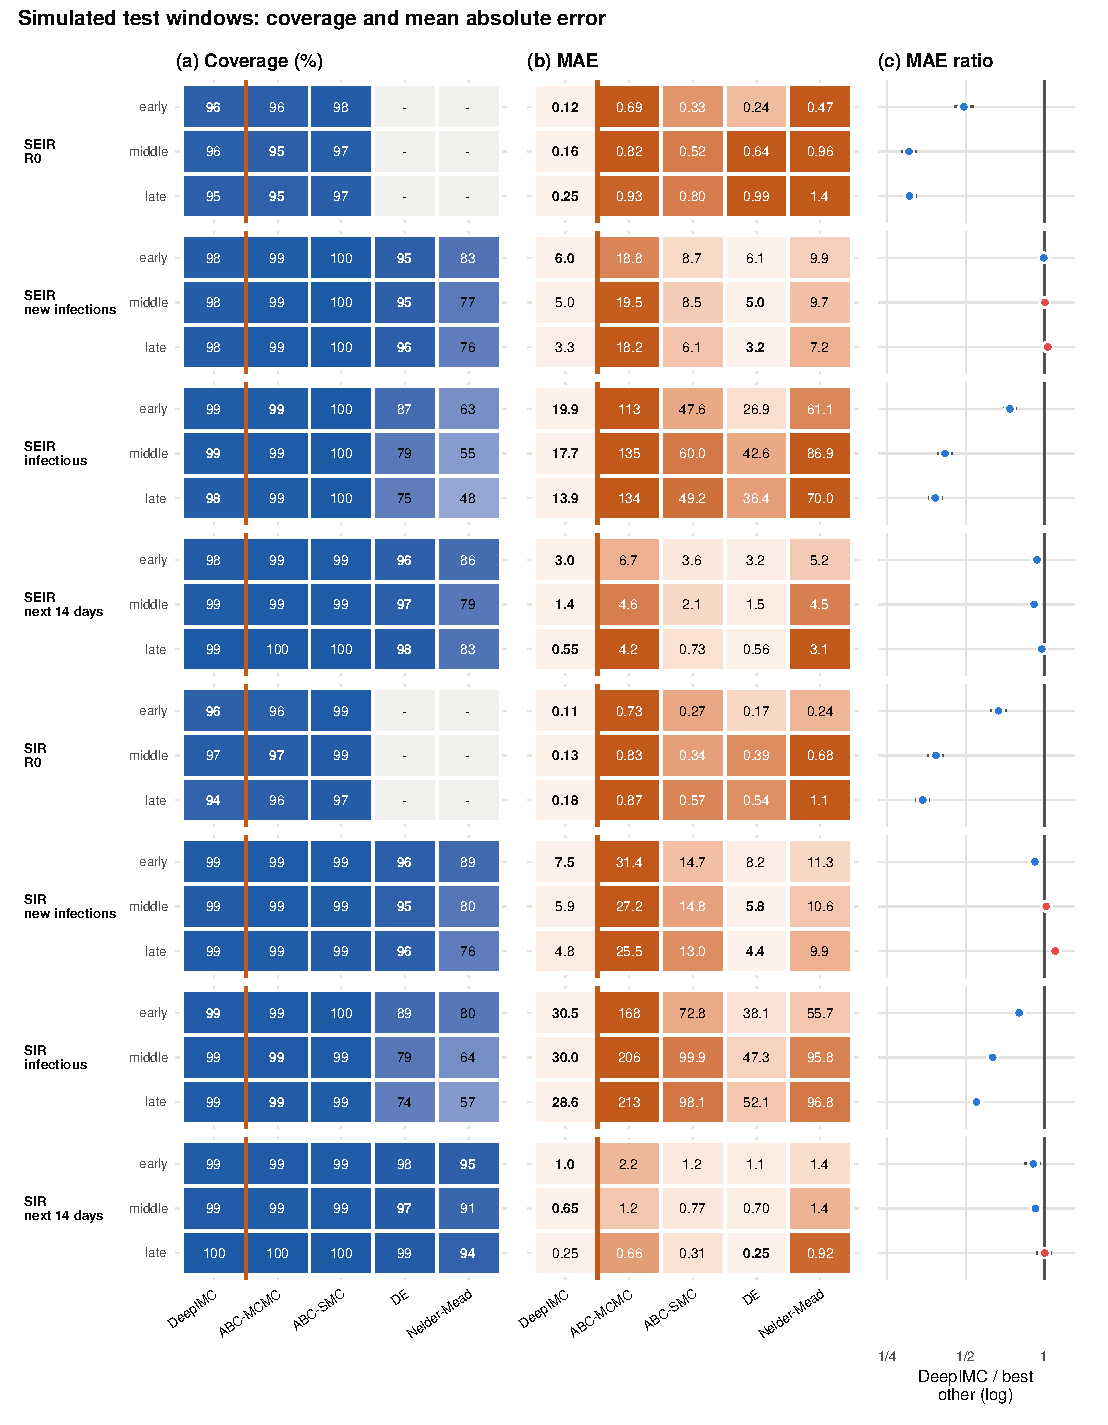
\includegraphics[width=\textwidth]{figures/coverage_mae_simulated.pdf}
\caption{Simulated test windows. (a) Mean coverage by method, for early, middle and late windows: of
the true $R_0$ by the 95\% range, and of the true curves by the 95\% band (bold: closest to 95\%;
``-'': the method gives no range). (b) Mean absolute error of $R_0$ and of the regenerated curves (bold:
lowest). (c) MAE of DeepIMC divided by that of the best comparison method for the same windows (log
scale; below 1: DeepIMC better), with 95\% paired bootstrap intervals.}
\label{fig:heatmap-sim}
\end{figure}

\begin{figure}[htbp]
\centering
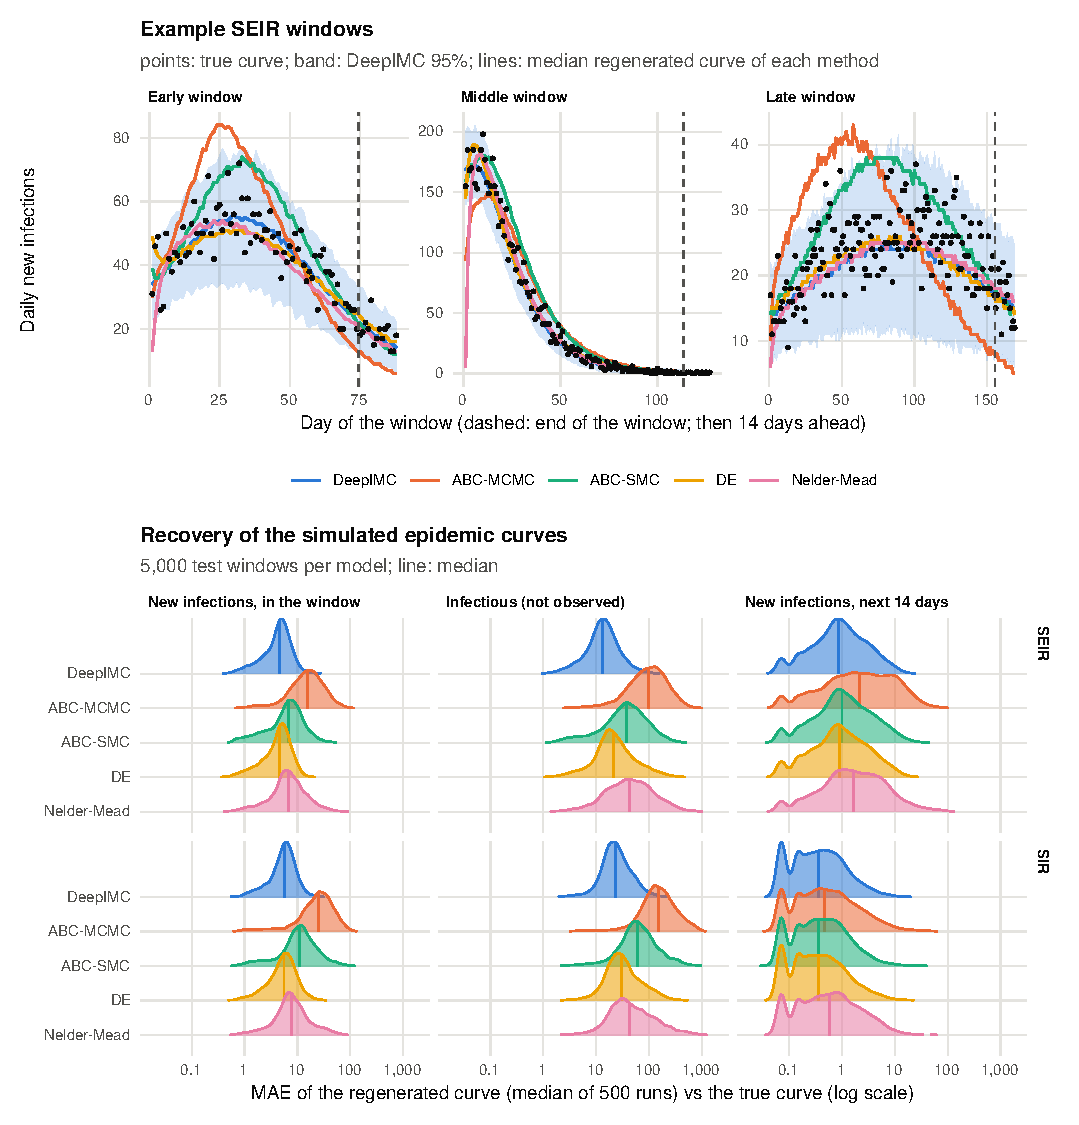
\includegraphics[width=\textwidth]{figures/curve_recovery.pdf}
\caption{Recovery of the simulated epidemic curves. Top: three SEIR test windows (early, middle and late)
with the true curve (points), DeepIMC's 95\% band and every method's median regenerated curve; the dashed
line marks the end of the window. Bottom: distribution over all test windows of the MAE of the median
regenerated curve (log scale; vertical line: median).}
\label{fig:curve-recovery}
\end{figure}

\begin{figure}[htbp]
\centering
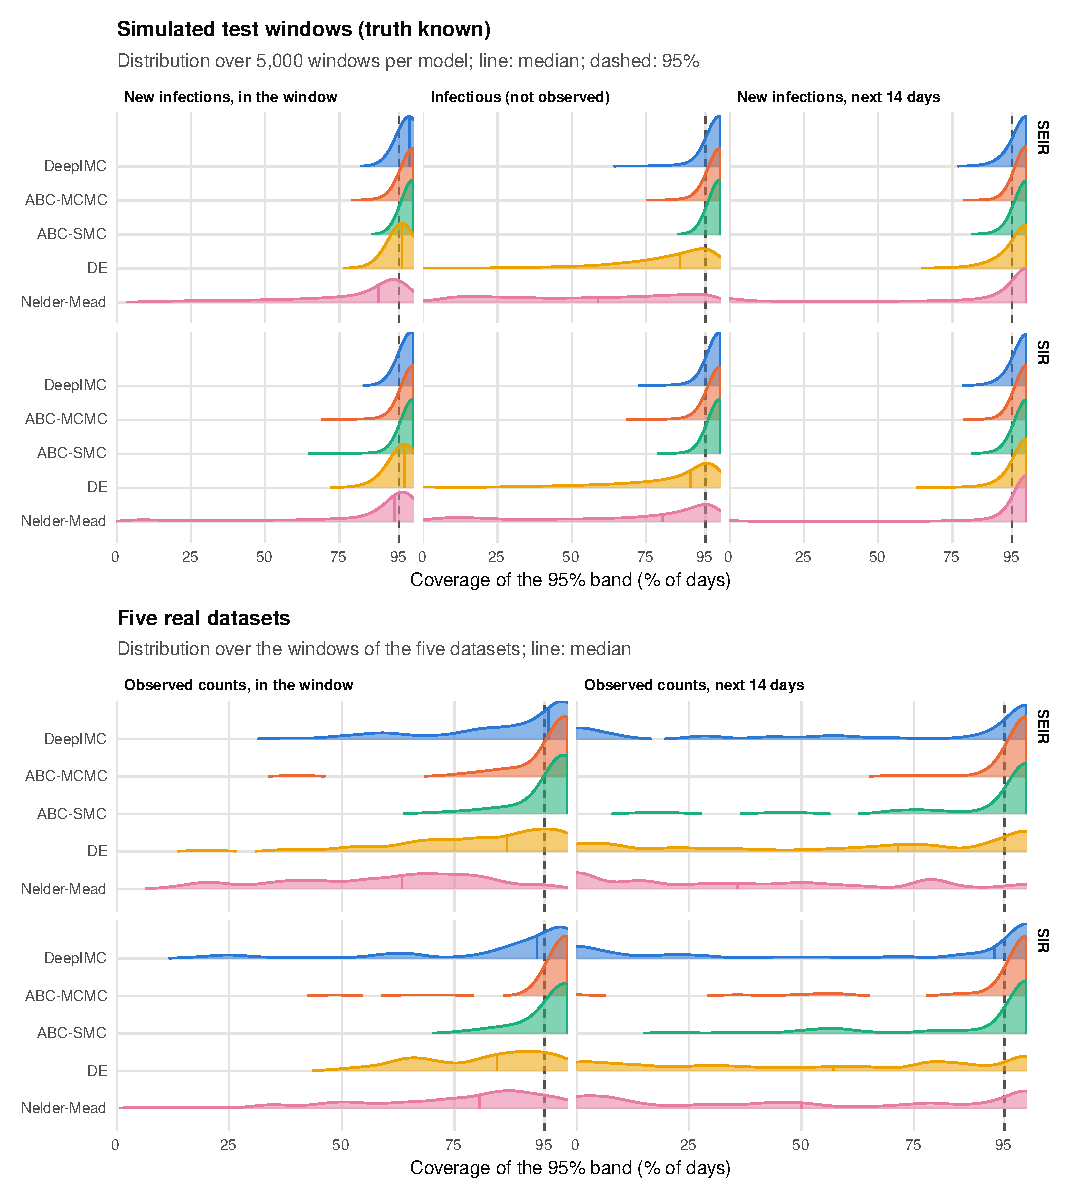
\includegraphics[width=\textwidth]{figures/coverage_ridgelines.pdf}
\caption{Distribution of the coverage of the 95\% band over the windows, by method: simulated test
windows (top) and the five real datasets (bottom). Vertical line in each ridge: median; dashed: 95\%.}
\label{fig:ridgelines}
\end{figure}

\subsection{Real data}\label{sec:res-real}

On real data the question is how well each method's regenerated curves match the observed counts, in the
window and over the following two weeks. Table~\ref{tab:real} and Figure~\ref{fig:heatmap-real} give the
coverage and the mean absolute error for each dataset.

\paragraph{Fit to the window.} DeepIMC's bands covered 77--100\% of the observed days, against 89--100\%
for the two ABC methods, 66--97\% for differential evolution and 42--90\% for Nelder--Mead. Coverage alone,
however, rewards wide bands: ABC-MCMC reached 90--100\% with bands so wide that its median curve was the
furthest from the data on most datasets. By the mean absolute error of the median curve, differential
evolution, which fits each window directly, came closest to the data on most datasets, and DeepIMC was
close to it on the influenza series, Baltimore 1918 and Ebola (Figure~\ref{fig:heatmap-real}). DeepIMC was
furthest behind on the Hong Kong SARS outbreak and on the Utah COVID-19 admissions.

\paragraph{By window length and position.} Figure~\ref{fig:methods-by-window-real} shows the same comparison by
window length (30, 60 and 90 days) and position. For most methods the coverage of the window fell as the window
grew longer, because a longer window is more likely to contain changes that a model with constant parameters cannot
follow; DeepIMC's coverage fell most, from 93--100\% for 30-day windows to 60--81\% for 90-day windows,
while its MAE stayed within a factor of two of the best method. The ABC methods kept their coverage with
wide bands, at the cost of the largest errors (ABC-MCMC up to 13 times the best).

\paragraph{The next 14 days.} Predicting the two weeks after a window was harder for every method. Thanks to
their wide bands the ABC methods covered most of these days, while DeepIMC covered 73--100\% of them for the
influenza series but only 42--52\% for the COVID-19 admissions and 32--64\% for the SARS and Ebola outbreaks
under the SEIR model (Table~\ref{tab:real-future}). By the MAE, differential evolution or ABC-SMC came
closest on most datasets; DeepIMC was close to them on the influenza series and furthest behind on the SARS
outbreak under the SEIR model. Figure~\ref{fig:real-examples} shows why: around the
peak of the SARS outbreak, DeepIMC continued the growth it saw in the window, while the outbreak, brought
under control, declined. A model with constant parameters within a window cannot anticipate such a change;
the comparison methods share this limitation, and their wider bands absorb more of it.

\paragraph{Estimated $R_0$.} The median estimates of $R_0$ for each dataset were between 1.0 and 2.1 for
DeepIMC, 1.2 and 2.1 for ABC-SMC and 1.1 and 3.6 for differential evolution. Those of ABC-MCMC (1.9 to 2.9)
stayed close to the middle of its prior range, a sign, as on simulated data, that its posterior was close to
the prior.

\paragraph{The contrast series.} The Utah COVID-19 cases by test report date are shown at the bottom of
Table~\ref{tab:real}. Scaled to cases per 10,000 residents, their daily counts are small (below 40), so
their coverage and errors cannot be compared directly with those of the admissions series of the same
waves.

\begin{table}[htbp]
\centering
\caption{Real data: coverage (\%) of the observed daily counts in the window by the 95\% band, and MAE of
the median regenerated curve, mean over the windows of each dataset (number of windows per model in
brackets). Bold: coverage closest to 95\% and lowest MAE. $^\dagger$Contrast series: cases by test report
date, per 10,000 residents.}
\label{tab:real}
\small
\resizebox{\textwidth}{!}{\begin{tabular}{llrrrrrrrrrr}
\toprule
 &  & \multicolumn{5}{c}{Coverage of the observed counts (\%)} & \multicolumn{5}{c}{MAE of the median curve} \\
\cmidrule(lr){3-7}\cmidrule(lr){8-12}
Dataset & Model & DeepIMC & ABC-MCMC & ABC-SMC & DE & Nelder--Mead & DeepIMC & ABC-MCMC & ABC-SMC & DE & Nelder--Mead \\
\midrule
Utah COVID-19 admissions (27) & SEIR & 85 & 100 & \textbf{98} & 82 & 71 & 12.7 & 24.9 & 13.4 & \textbf{9.5} & 12.1 \\
 & SIR & 77 & 100 & \textbf{96} & 81 & 79 & 17.2 & 24.6 & 14.6 & \textbf{10.8} & 11.4 \\
Utah influenza admissions (18) & SEIR & 100 & \textbf{95} & 100 & 97 & 46 & 2.2 & 26.5 & 3.3 & \textbf{2.2} & 3.0 \\
 & SIR & \textbf{96} & 98 & 100 & 88 & 90 & 2.5 & 15.8 & 4.2 & \textbf{2.2} & 2.2 \\
Baltimore influenza 1918 (9) & SEIR & 85 & 92 & \textbf{95} & 66 & 42 & 36.2 & 76.9 & 34.6 & \textbf{32.6} & 41.4 \\
 & SIR & 88 & 90 & \textbf{95} & 81 & 44 & 32.3 & 74.9 & 48.9 & \textbf{30.3} & 50.4 \\
Hong Kong SARS 2003 (9) & SEIR & 78 & \textbf{91} & 89 & 67 & 59 & 24.2 & 30.1 & 10.8 & \textbf{8.8} & 10.1 \\
 & SIR & 81 & 100 & \textbf{93} & 73 & 60 & 10.9 & 18.7 & 10.6 & \textbf{8.4} & 10.4 \\
Sierra Leone Ebola 2014-15 (9) & SEIR & 84 & 99 & \textbf{96} & 74 & 65 & 7.8 & 18.4 & 9.2 & \textbf{6.9} & 7.9 \\
 & SIR & 88 & 100 & \textbf{98} & 77 & 73 & 8.4 & 15.2 & 8.2 & \textbf{7.2} & 8.2 \\
Utah COVID-19 cases$^\dagger$ (27) & SEIR & \textbf{96} & 100 & 100 & 91 & 81 & 4.8 & 15.5 & 3.2 & \textbf{2.8} & 3.4 \\
 & SIR & \textbf{97} & 100 & 100 & 90 & 88 & 3.6 & 8.9 & \textbf{3.2} & 3.3 & 3.5 \\
\bottomrule
\end{tabular}
}
\end{table}

\begin{table}[htbp]
\centering
\caption{Real data: coverage (\%) of the observed counts in the 14 days after the window (where the
data continue) and MAE of the median regenerated curve over those days. Bold: coverage closest to 95\% and
lowest MAE.}
\label{tab:real-future}
\small
\resizebox{\textwidth}{!}{\begin{tabular}{llrrrrrrrrrr}
\toprule
 &  & \multicolumn{5}{c}{Coverage, next 14 days (\%)} & \multicolumn{5}{c}{MAE, next 14 days} \\
\cmidrule(lr){3-7}\cmidrule(lr){8-12}
Dataset & Model & DeepIMC & ABC-MCMC & ABC-SMC & DE & Nelder--Mead & DeepIMC & ABC-MCMC & ABC-SMC & DE & Nelder--Mead \\
\midrule
Utah COVID-19 admissions & SEIR & 52 & 98 & \textbf{93} & 47 & 32 & 22.6 & 30.2 & \textbf{17.7} & 18.5 & 24.2 \\
 & SIR & 42 & \textbf{92} & 88 & 34 & 29 & 27.1 & 35.6 & \textbf{21.6} & 23.6 & 25.6 \\
Utah influenza admissions & SEIR & 100 & 100 & 100 & \textbf{95} & 48 & 2.1 & 3.1 & 2.4 & 3.6 & \textbf{1.7} \\
 & SIR & 93 & \textbf{94} & 100 & 82 & 87 & 1.7 & 1.6 & 1.5 & \textbf{1.5} & 2.1 \\
Baltimore influenza 1918 & SEIR & 87 & \textbf{98} & 99 & 75 & 58 & 32.6 & 44.0 & 31.0 & \textbf{29.3} & 48.1 \\
 & SIR & 73 & \textbf{95} & 96 & 81 & 73 & 42.6 & 41.2 & 34.0 & \textbf{24.9} & 36.2 \\
Hong Kong SARS 2003 & SEIR & 32 & \textbf{100} & 77 & 25 & 17 & 93.4 & \textbf{14.9} & 28.5 & 29.3 & 17.3 \\
 & SIR & 98 & 100 & \textbf{93} & 39 & 30 & 15.2 & \textbf{11.2} & 21.2 & 14.1 & 12.8 \\
Sierra Leone Ebola 2014-15 & SEIR & 64 & \textbf{100} & 81 & 58 & 36 & 16.1 & 30.0 & 18.7 & \textbf{12.5} & 16.3 \\
 & SIR & 62 & \textbf{100} & 77 & 57 & 49 & 17.0 & 29.3 & 18.6 & \textbf{12.8} & 17.7 \\
Utah COVID-19 cases & SEIR & 87 & 100 & \textbf{98} & 80 & 61 & 12.8 & 5.3 & \textbf{3.5} & 5.0 & 5.3 \\
 & SIR & 100 & 100 & \textbf{99} & 79 & 65 & 4.5 & \textbf{3.4} & 3.6 & 6.5 & 5.7 \\
\bottomrule
\end{tabular}
}
\end{table}

\begin{figure}[htbp]
\centering
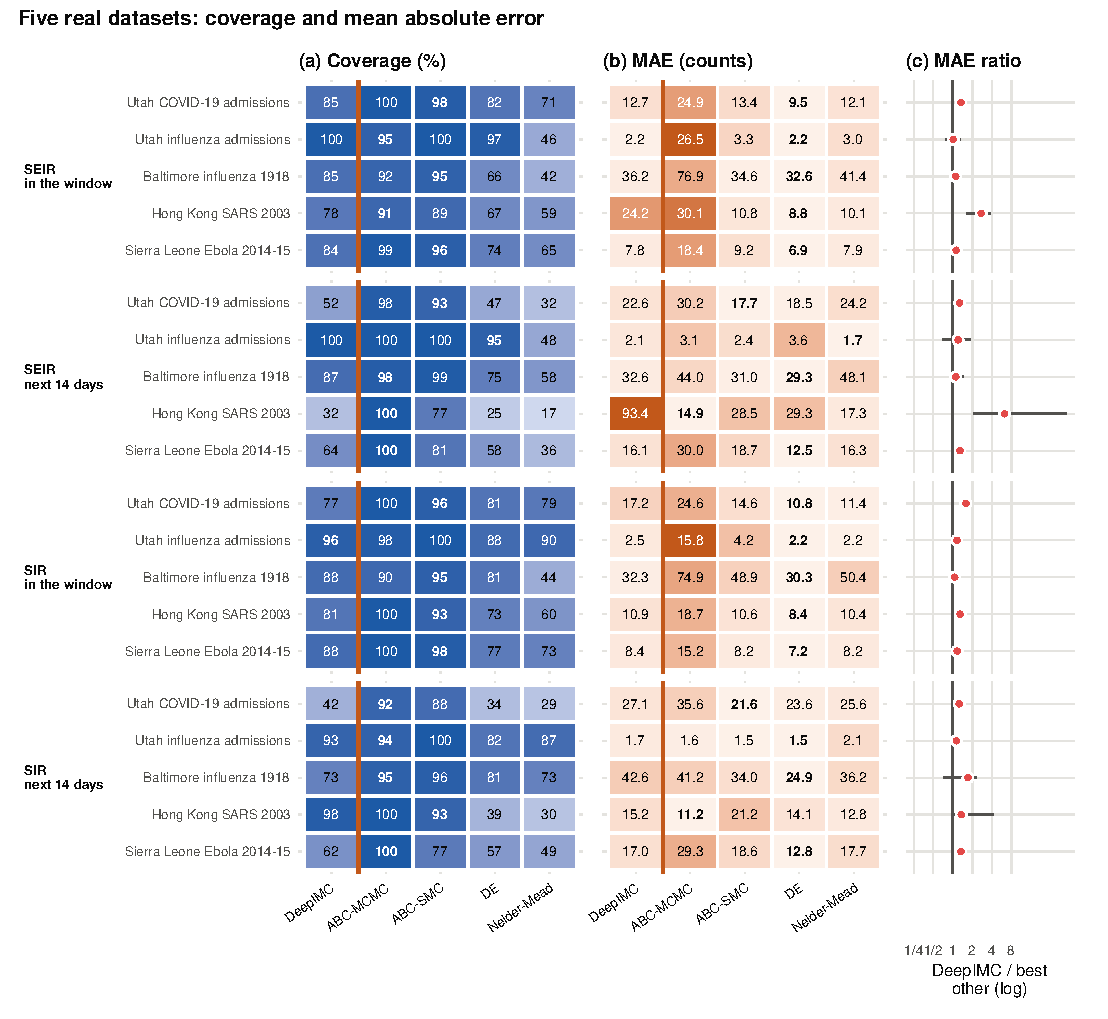
\includegraphics[width=\textwidth]{figures/coverage_mae_real.pdf}
\caption{Real data. (a) Mean coverage of the 95\% band of each method, for each dataset and model, in the
window and in the 14 days after it (bold: closest to 95\%). (b) Mean absolute error of the median
regenerated curve, in daily counts (bold: lowest). (c) MAE of DeepIMC divided by that of the best
comparison method for the same windows (log scale; below 1: DeepIMC better), with 95\% paired bootstrap
intervals.}
\label{fig:heatmap-real}
\end{figure}

\begin{figure}[htbp]
\centering
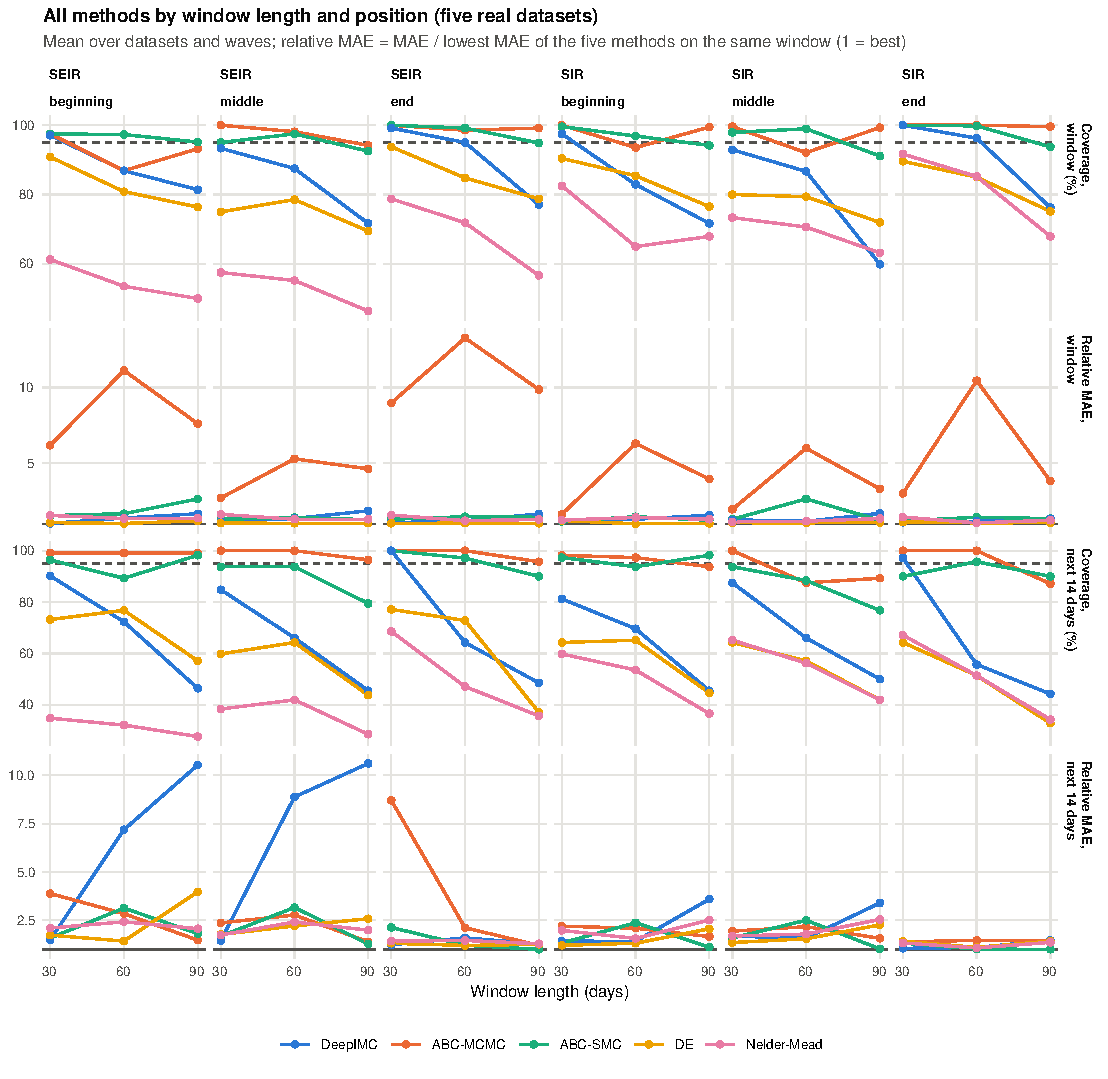
\includegraphics[width=\textwidth]{figures/methods_by_window_real.pdf}
\caption{All methods on the five real datasets, by window length and position: coverage of the observed counts
by the 95\% band and relative MAE of the median regenerated curve (the MAE divided by the lowest MAE of the five
methods on the same window, so that datasets of different size can be averaged; 1 is best), in the window and
in the 14 days after it.}
\label{fig:methods-by-window-real}
\end{figure}

\begin{figure}[htbp]
\centering
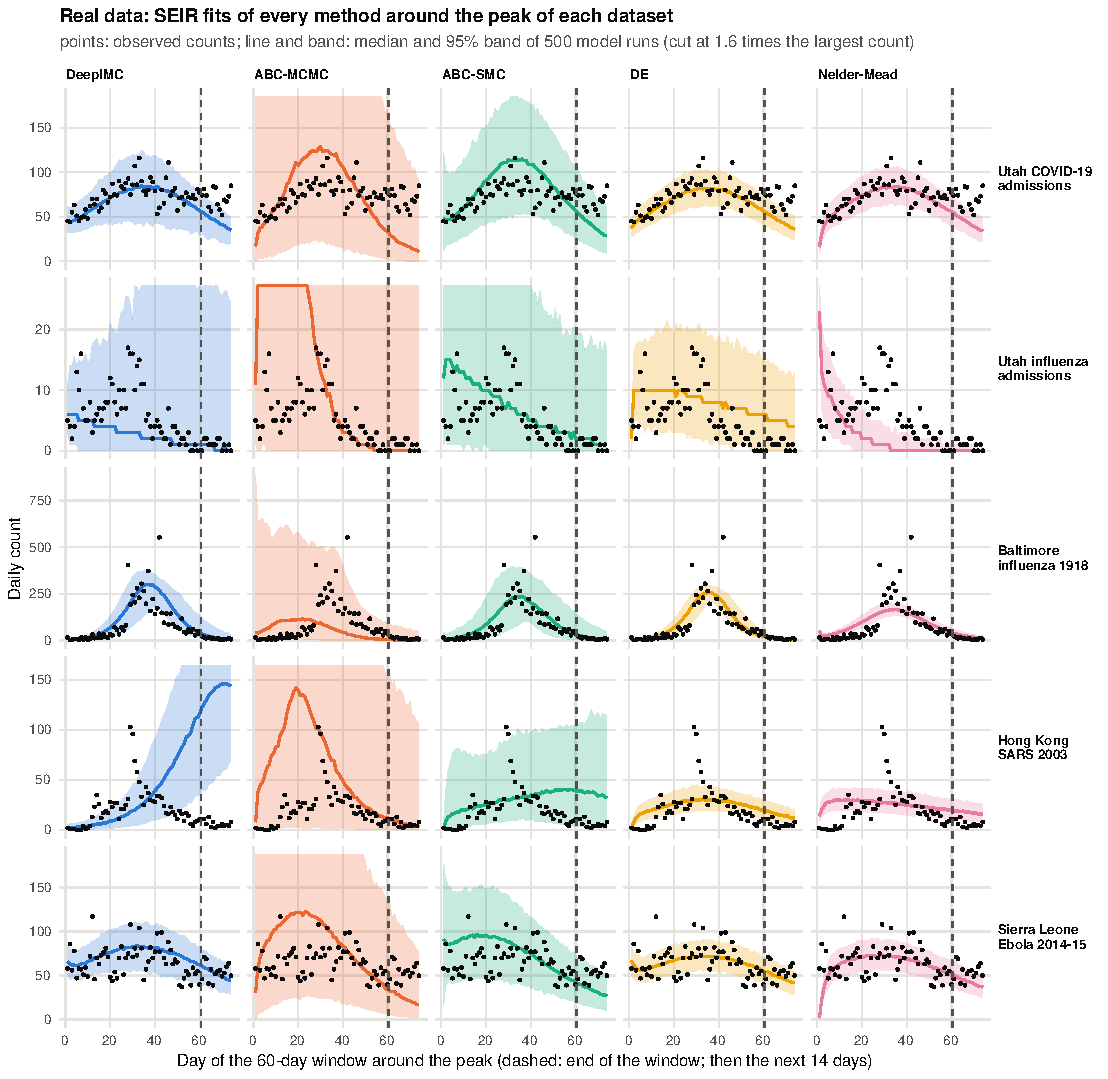
\includegraphics[width=\textwidth]{figures/real_examples.pdf}
\caption{Real data: SEIR fits of every method to the 60-day window in the middle of each dataset, with the next
14 days (after the dashed line). Points: observed counts; lines and bands: median and 95\% band of 500 model
runs from each method's estimates (cut at 1.6 times the largest observed count). The SIR fits are in
Figure~\ref{fig:real-examples-sir}.}
\label{fig:real-examples}
\end{figure}

\subsection{Computing time}\label{sec:res-cost}

The last question is what each method costs. Table~\ref{tab:timing} separates the cost of calibrating a
new window from DeepIMC's one-time cost of training.

\paragraph{Calibrating a window.} On one CPU core, DeepIMC calibrated a window in 0.14 seconds (SEIR) and
0.10 seconds (SIR), and slightly less per window when several windows were processed together. Its first
call in an R session took 10 and 6.5 seconds, almost all of it to start Python and load the five
networks; this is paid once per session. The comparison methods took between 3.6 seconds (Nelder--Mead,
SIR) and 536 seconds (differential evolution, SEIR) per window. For SEIR windows, DeepIMC was about 1,400
times faster than ABC-MCMC, 2,800 times faster than ABC-SMC and 3,800 times faster than differential
evolution; it was 70 times faster than Nelder--Mead, the cheapest of the comparison methods.

\paragraph{From a fit to a band.} Turning a fit into a 95\% band with 500 runs of the agent-based model
took 32 (SEIR) and 17 (SIR) seconds per window, far longer than DeepIMC's fit itself. The renewal equation
gave a band in 0.18 and 0.11 seconds.

\paragraph{The one-time cost.} Simulating the 1,000,000 training epidemics took 30 (SEIR) and 14 (SIR)
CPU-hours, and computing DeepIMC's estimates for the 100,000 calibration windows of the $R_0$ range 1.5 and
0.2 hours on one core. Training is the largest part: one SEIR network would need about 85 hours on 16 CPU
cores (30 hours for SIR), which is why we trained on GPUs, where one network took 3.7 to 20 hours depending
on the GPU. The simulation time alone equals the cost of calibrating about 200 SEIR windows with
differential evolution or 270 with ABC-SMC; with training on CPUs, the one-time cost equals tens of
thousands of windows. It is paid once, by the developer: the trained networks are shipped with the
package, and its users pay only the cost of a calibration.

\begin{table}[htbp]
\centering
\caption{Computing time on CPUs (one core per method, the same computer for all methods), and the
one-time cost of DeepIMC.}
\label{tab:timing}
\small
\begin{tabular}{lrr}
\toprule
 & SEIR & SIR \\
\midrule
\multicolumn{3}{l}{\textit{Calibrating one window (seconds, one CPU core)}} \\
DeepIMC, first call (starts Python, loads networks) & 10.1 & 6.5 \\
DeepIMC, one window & 0.142 & 0.099 \\
DeepIMC, 10 windows in one pass, per window & 0.120 & 0.065 \\
ABC-MCMC & 199.9 & 93.2 \\
ABC-SMC & 397.4 & 131.8 \\
DE & 536.5 & 203.1 \\
Nelder--Mead & 10.0 & 3.6 \\
\midrule
\multicolumn{3}{l}{\textit{From a fit to a 95\% band (seconds per window)}} \\
500 runs of the agent-based model & 32.3 & 16.6 \\
Renewal equation & 0.179 & 0.109 \\
\midrule
\multicolumn{3}{l}{\textit{One-time cost of DeepIMC (CPU)}} \\
Simulating 1,000,000 training epidemics (CPU-hours) & 29.6 & 14.1 \\
Estimates for 100,000 calibration windows (hours, 1 core) & 1.5 & 0.2 \\
Training one network, 50 epochs (hours, 16 cores, estimated) & 84.9 & 29.6 \\
\midrule
\multicolumn{3}{l}{\textit{For reference: training as done, on GPUs}} \\
Training one network, 50 epochs (hours, one GPU) & 3.7--20.4 & 2.6--9.9 \\
\bottomrule
\end{tabular}

\end{table}

% =============================================================================
\section{Discussion}\label{sec:discussion}

We introduced DeepIMC, a neural network that maps a window of daily new infections of any length, from
any part of an epidemic, to the basic reproduction number and the current state of an agent-based SEIR or
SIR epidemic. On 10,000 simulated test windows, where the truth is known, it estimated $R_0$ about three
times more accurately than four standard calibration methods used with their default settings. Its ranges
for $R_0$ had close to nominal coverage while being far narrower than those of ABC; it recovered the state of
the epidemic, and the number of infectious people that no method observes, better than every other method;
and it calibrated a window in a fraction of a second on one CPU core. On real data the comparison was closer,
and depended on how closely each dataset matched the model.

\subsection{What the curve can and cannot tell}

The transmission probability and the contact rate cannot be separated from a curve of daily
infections, by DeepIMC or by any other method: their errors equal those of a guess that knows $R_0$
exactly, because only their product shapes the epidemic. This does not limit the use of a calibrated
model for prediction, which depends on $R_0$ and the current state; but estimating $p_{tran}$ and
$c_{rate}$ separately requires additional information, such as contact rates from a contact survey.

\subsection{Why DeepIMC is more accurate}

At the beginning of an epidemic, the growth of the curve reveals $R_0$ almost directly, and differential
evolution came closest to DeepIMC. In the middle and at the end of an epidemic, a method must also find
how many people are already infected or immune, and many combinations of $R_0$ and starting state produce
similar curves. The comparison methods search this space by trial and error, over thousands of stochastic
simulations, for every window; DeepIMC has learned from a million simulated epidemics which combinations are
likely, and this is where its advantage was largest.

The comparison methods failed in different ways. Differential evolution matched the observed curve as closely
as DeepIMC, because it fits each window directly, but its single estimate could not express how uncertain the
starting state is, and its estimate of the unobserved number of infectious people was twice as far from the
truth. ABC-MCMC, with its tolerance set from 200 simulations from the prior, stayed close to the prior: its
estimates were pulled towards the middle of the range and its ranges covered most of it. ABC-SMC was the most
accurate comparison method for SEIR windows but still underestimated many large values of $R_0$. Nelder--Mead
was the weakest method on the curves: with a fixed-seed agent-based model the fit is flat and irregular, so its
stopping rule is met after about 100 runs, often far from the best values.

\subsection{Ease of use}

DeepIMC needs only the daily counts and the known values. Each comparison method required choices
before it could be used: ranges for $R_0$ and for the starting state, how to parameterize them, the
number of model runs, tolerances and, for ABC, the summary statistics and their scaling. Even with
default settings, ABC-SMC failed on most SEIR windows until its limits were raised. These choices
are made once, by the developer, when DeepIMC is trained; users of the trained models do not face them.

\subsection{Real data and the choice of data}

DeepIMC was trained on noise-free epidemics, in which every new infection is counted, in a closed
population with constant parameters. Real data depart from these assumptions in three ways: only a
fraction of infections is recorded, the recorded counts depend on testing and reporting, and the course
of an epidemic changes with behaviour and interventions. The choice of data therefore matters. Counts by
date of symptom onset and hospital admissions by date of admission follow new infections more closely
than cases by date of report, which follow the reporting week and the availability of tests. On the
datasets closest to the model's assumptions---influenza waves recorded by admission or onset, and the
Ebola outbreak---DeepIMC fitted the data almost as closely as the best comparison method, in a fraction of
a second. On outbreaks that were brought under control, such as SARS in Hong Kong, no method with
constant parameters can follow the decline, and DeepIMC, whose bands are narrower, was penalized most.

A version of DeepIMC trained on simulated \emph{reported} cases, with a reported share of infections,
weekday effects and extra noise, is a natural way to close this gap. In earlier experiments with 61-day
windows, such a version raised the coverage of 24 Utah COVID-19 case-report windows from 46\% to 69\%: an
improvement, but not enough to match the methods that fit each curve directly on data that also change
over time in ways a model with constant parameters cannot follow.

\subsection{Computational efficiency}

Because DeepIMC calibrates a window in a fraction of a second on an ordinary CPU, it can be used where the
standard methods are impractical: for many locations at once, every day of an ongoing outbreak as new
data arrive, or inside a larger analysis that calibrates thousands of windows, such as the evaluation in
this paper. The cost is moved to training, which in practice needs a GPU and is paid once for each model
structure and range of parameters. For a model that will be calibrated only a few times, a standard
method is cheaper; for a model that is calibrated repeatedly, as in surveillance or by the many users of
a shipped model, the one-time cost is soon recovered. Once the calibration takes a fraction of a second,
the slowest step of a prediction is the simulation of the band.

The renewal equation reduces that step to a fraction of a second (Appendix~\ref{sec:res-renewal}): started from
DeepIMC's estimated state, it
gave nearly the same curves of new infections as 500 model runs, about 180 times faster, at the price of bands for the
number currently infectious that are too narrow.
\subsection{Limitations}

The models assume homogeneous mixing, parameters that are constant within a window, and a known
population size, recovery rate and latent period. Real population sizes must be mapped to the trained
range, and the reported fraction of infections cannot be separated from the population size. The trained
ranges of Table~\ref{tab:priors} bound the epidemics the shipped models can calibrate: the shortest
infectious period is 4 days, longer than that of influenza, so influenza is represented with a longer
generation interval than observed. Other settings require new training data and retraining, which the
software supports. Finally, the $R_0$ ranges are calibrated empirically on simulated windows rather than
derived from a posterior distribution.

\subsection{Future work}

Training DeepIMC on simulated reported data---with a reported fraction of infections, a weekly reporting
pattern and extra noise---would let it read case reports directly. Parameters that change over time,
other contact structures such as networks, and models with hospitalization are natural extensions; the
same training code applies to any model that can be simulated.

% =============================================================================
\section{Conclusions}

Calibrating agent-based models is computationally demanding and requires many choices from the user.
DeepIMC reverses the usual approach: it learns, once, the inverse mapping from epidemic curves to the
quantities that generated them, using data simulated from the model itself. For agent-based SEIR and SIR
models, it estimates $R_0$ and the current state of an epidemic from a window of any length and position,
reproduces the epidemic those estimates imply, and answers in a fraction of a second on an ordinary CPU,
with no settings to choose. How well it does on real data depends on how closely the data resemble the
simulations it was trained on, which makes the choice of data---onset dates and admissions rather than
reported cases---as important as the choice of method.

% =============================================================================
\section{Software availability}

The R package \texttt{epiworldRcalibrate} provides:
\begin{itemize}
\item the trained SEIR and SIR calibrators: \texttt{window\_calibrator()} and \texttt{calibrate()};
\item the four comparison methods, set up as in this paper: \texttt{window\_baselines()}, with
\texttt{epidemic\_summary()} for the summary statistics of the ABC methods;
\item predictions by model simulation or the renewal equation: \texttt{predict\_cases()};
\item the evaluation scores: \texttt{coverage()}, \texttt{interval\_score()} and \texttt{score\_band()};
\item the comparison of methods on many windows: \texttt{compare\_methods()};
\item simulation of training data, tuning and training of new calibrators:
  \texttt{simulate\_window\_data()}, \texttt{tune\_window\_calibrator()} and
  \texttt{train\_window\_calibrator()}.
\end{itemize}
All code needed to reproduce the results is available at: repository link removed for double-blind review.

\section*{Acknowledgments}
Acknowledgments removed for double-blind review.

\printbibliography

% =============================================================================
\appendix

\section{Simulation details}\label{sec:sim-parameters}

Epidemics were simulated with \texttt{ModelSEIRCONN} and \texttt{ModelSIRCONN} of \textbf{epiworldR} for
365 days with the distributions of Table~\ref{tab:priors}. A new epidemic starts with the drawn share of
the population exposed (SEIR) or infectious (SIR) and nobody recovered. The daily count is the number of
transitions from exposed to infectious (SEIR) or from susceptible to infectious (SIR); the shares in each
state are recorded at the start of each day, so the state at the start of a window is the state at the
start of its first day. Separate sets were simulated for training (1,000,000 epidemics per model, 80\% for
training and 20\% for validation), for the calibration windows of the $R_0$ range (100,000), for the test
of DeepIMC by window length (1,000) and for the comparison with the other methods (10,000 in all).

\section{Network and training details}\label{app:training}

\begin{table}[htbp]
\centering
\caption{Settings of the two DeepIMC models. The search space of the hyperparameter search is given in
brackets.}
\label{tab:hyper}
\small
\resizebox{\textwidth}{!}{%
\begin{tabular}{lll}
\toprule
Setting & SEIR & SIR \\
\midrule
BiLSTM layers [1--3] & 3 & 2 \\
Hidden units per direction [64, 128, 160, 256] & 128 & 64 \\
Dropout between layers [0--0.5] & 0.13 & 0.28 \\
Initial learning rate [$10^{-4}$--$10^{-3}$, log scale] & $7.16\times10^{-4}$ & $7.94\times10^{-4}$ \\
Batch size [32, 64, 128, 256] & 32 & 32 \\
Learning-rate schedule & cosine, to 1\% over 50 epochs & same \\
Gradient-norm clipping & 1 & 1 \\
Dense layer & 64 units, ReLU & same \\
Output activations & sigmoid ($p_{tran}$, shares), softplus ($R_0$) & same \\
Networks averaged & 5 & 5 \\
\bottomrule
\end{tabular}}
\end{table}

The hyperparameter search used Optuna's tree-structured Parzen estimator with a median pruner (trials worse
than the median of earlier trials after 5 epochs were stopped). Each trial trained one network for 20 epochs
on 100,000 training epidemics and was scored by the validation mean squared error, half for $R_0$ and half
for the state shares. The best settings (Table~\ref{tab:hyper}) improved the validation score by 3\% (SEIR)
and 5\% (SIR) over the settings of an earlier model.

Table~\ref{tab:versions} compares three versions of the networks on the same test windows. \emph{Current}
uses the settings of the earlier model, 300,000 training epidemics and 100 epochs with a constant learning
rate; \emph{Tuned} uses the settings of Table~\ref{tab:hyper}, otherwise as Current; \emph{Final}, the
version used in this paper, uses the tuned settings, 1,000,000 epidemics and the cosine learning-rate
schedule over 50 epochs. Tuning alone changed the test errors little; more training data and the
decreasing learning rate reduced the $R_0$ error further. As expected, no version improved $p_{tran}$ or
$c_{rate}$, which the curves do not reveal.

\begin{table}[htbp]
\centering
\caption{Mean absolute error of $R_0$, $p_{tran}$ and $c_{rate}$ of three versions of the networks (5
networks each) on the same test windows: 61-day windows from the beginning of the test epidemics, and all
test windows (lengths 30--365 days at the beginning, middle and end).}
\label{tab:versions}
\small
\begin{tabular}{llrrrrrr}
\toprule
 &  & \multicolumn{3}{c}{61-day windows from the beginning} & \multicolumn{3}{c}{All test windows} \\
\cmidrule(lr){3-5}\cmidrule(lr){6-8}
Model & Version & $R_0$ & $p_{tran}$ & $c_{rate}$ & $R_0$ & $p_{tran}$ & $c_{rate}$ \\
\midrule
SEIR & Current & 0.121 & 0.0145 & 2.58 & 0.223 & 0.0141 & 2.56 \\
 & Tuned & 0.118 & 0.0147 & 2.60 & 0.225 & 0.0141 & 2.57 \\
 & Final & 0.107 & 0.0145 & 2.59 & 0.218 & 0.0141 & 2.57 \\
\midrule
SIR & Current & 0.109 & 0.0483 & 1.06 & 0.192 & 0.0524 & 1.05 \\
 & Tuned & 0.106 & 0.0490 & 1.08 & 0.195 & 0.0532 & 1.07 \\
 & Final & 0.098 & 0.0486 & 1.07 & 0.189 & 0.0527 & 1.06 \\
\bottomrule
\end{tabular}

\end{table}

\section{Comparison methods}\label{app:baselines}

All four methods search $\vartheta = (R_0, \log_{10} e_0, \log_{10} i_0, \log_{10} r_0)$ for SEIR and
$(R_0, \log_{10} i_0, \log_{10} r_0)$ for SIR, where $e_0$, $i_0$ and $r_0$ are the shares exposed,
infectious and recovered on the first day of the window, within $R_0\in[0.8, 5]$,
$\log_{10} e_0, \log_{10} i_0 \in [-4, \log_{10} 0.4]$ and $\log_{10} r_0 \in [-4, \log_{10} 0.95]$. If the
shares add up to more than 0.95 they are scaled down to 0.95. The contact rate is fixed at the middle of its
training range (10 for SEIR, 3 for SIR) and $p_{tran} = R_0\, p_{recov}/c_{rate}$. For a candidate
$\vartheta$, the model is run for the length of the window from the candidate state, and its daily new
infectious people $\hat y_t(\vartheta)$ are compared with the observed counts $y_t$: by
$\sum_t (y_t - \hat y_t(\vartheta))^2$ for DE and Nelder--Mead, and through summary statistics for the ABC
methods.

\paragraph{Summary statistics.} For a curve $x_1,\dots,x_T$: $\log(1+\bar x)$, $\log(1+\max_t x_t)$,
$\log(1+\min_t x_t)$, the day of the maximum of the centred 7-day average, $\log(1+\cdot)$ of the mean of
the first and of the last 7 days, the first days on which the cumulative count reaches 25\%, 50\% and 75\%
of $\sum_t x_t$, and the least-squares slopes of $\log(1+x_t)$ against $t$ over the first and the last 14
days (function \texttt{epidemic\_summary()} of the package). With $s(\cdot)$ the vector of statistics and
$\sigma_k$ the median absolute deviation of statistic $k$ over simulations from the prior, the distance is
$d = \big(\frac1K\sum_k [(s_k(\hat y)-s_k(y))/\sigma_k]^2\big)^{1/2}$.

\paragraph{ABC-MCMC.} 200 simulations from the prior give $\sigma_k$ and the tolerance $\varepsilon$, the 5\%
quantile of their distances; Gaussian random-walk proposals with standard deviation 8\% of each range,
uniform prior on the box, Gaussian kernel $\exp(-d^2/2\varepsilon^2)$, starting at the middle of the box;
3,000 steps, the last 1,500 kept; estimates are posterior medians and the $R_0$ range the 2.5\% and 97.5\%
posterior quantiles.

\paragraph{ABC-SMC.} 200 particles over 6 generations; the first generation, drawn from the prior, gives
$\sigma_k$; each tolerance is the median distance of the previous generation; perturbation by a
multivariate normal kernel with twice the weighted covariance of the particles; at most 30,000 model runs
and 20,000 attempts per generation.

\paragraph{DE.} \texttt{DEoptim} with strategy 2 (DE/local-to-best/1/bin), population $10 \times$ the number
of unknowns, $F = 0.8$, $CR = 0.5$, 200 generations.

\paragraph{Nelder--Mead.} \texttt{stats::optim} with its default settings (relative tolerance
$\approx 1.5\times10^{-8}$, at most 500 function evaluations), started at the middle of the box; candidates
outside the box receive an infinite fit.

\section{ABC on the whole curve or on summary statistics}\label{app:abc-sensitivity}

The ABC methods were also run comparing the whole curve day by day (root mean squared error, with
ABC-MCMC's tolerance $0.30\times$ the root mean square of the observed counts) on the 216 windows of an
earlier design (9 test epidemics for each model, window length of 30, 61, 120 and 180 days, and position at
the beginning, middle and end of the epidemic). Table~\ref{tab:abc-sensitivity} compares the two versions on
the same windows. With default settings, ABC-SMC gave similar results either way, while ABC-MCMC was less
accurate on summary statistics, mainly because its fixed tolerance, set from 200 prior simulations, was
loose.

\begin{table}[htbp]
\centering
\caption{ABC on the whole curve or on summary statistics, on the same 216 simulated windows: $R_0$ mean
absolute error, starting-state error (percentage points), and coverage and MAE of the true
daily new infections in the window.}
\label{tab:abc-sensitivity}
\small
\resizebox{\textwidth}{!}{\begin{tabular}{lllrrrrr}
\toprule
Model & Method & Compares & $R_0$ MAE & State error & Coverage (\%) & MAE & Seconds \\
\midrule
SEIR & ABC-MCMC & whole curve & 0.78 & 9.3 & 99.2 & 8.7 & 73 \\
 & ABC-MCMC & summary statistics & 0.95 & 10.0 & 98.7 & 15.7 & 143 \\
 & ABC-SMC & whole curve & 0.65 & 7.7 & 99.1 & 4.9 & 306 \\
 & ABC-SMC & summary statistics & 0.61 & 6.2 & 99.6 & 6.5 & 292 \\
\midrule
SIR & ABC-MCMC & whole curve & 0.56 & 7.8 & 99.3 & 9.7 & 56 \\
 & ABC-MCMC & summary statistics & 1.13 & 9.7 & 96.8 & 19.7 & 92 \\
 & ABC-SMC & whole curve & 0.39 & 7.0 & 99.2 & 7.0 & 169 \\
 & ABC-SMC & summary statistics & 0.42 & 5.5 & 99.6 & 8.8 & 171 \\
\bottomrule
\end{tabular}
}
\end{table}

\section{Real data: SIR fits}\label{app:real-sir}

\begin{figure}[htbp]
\centering
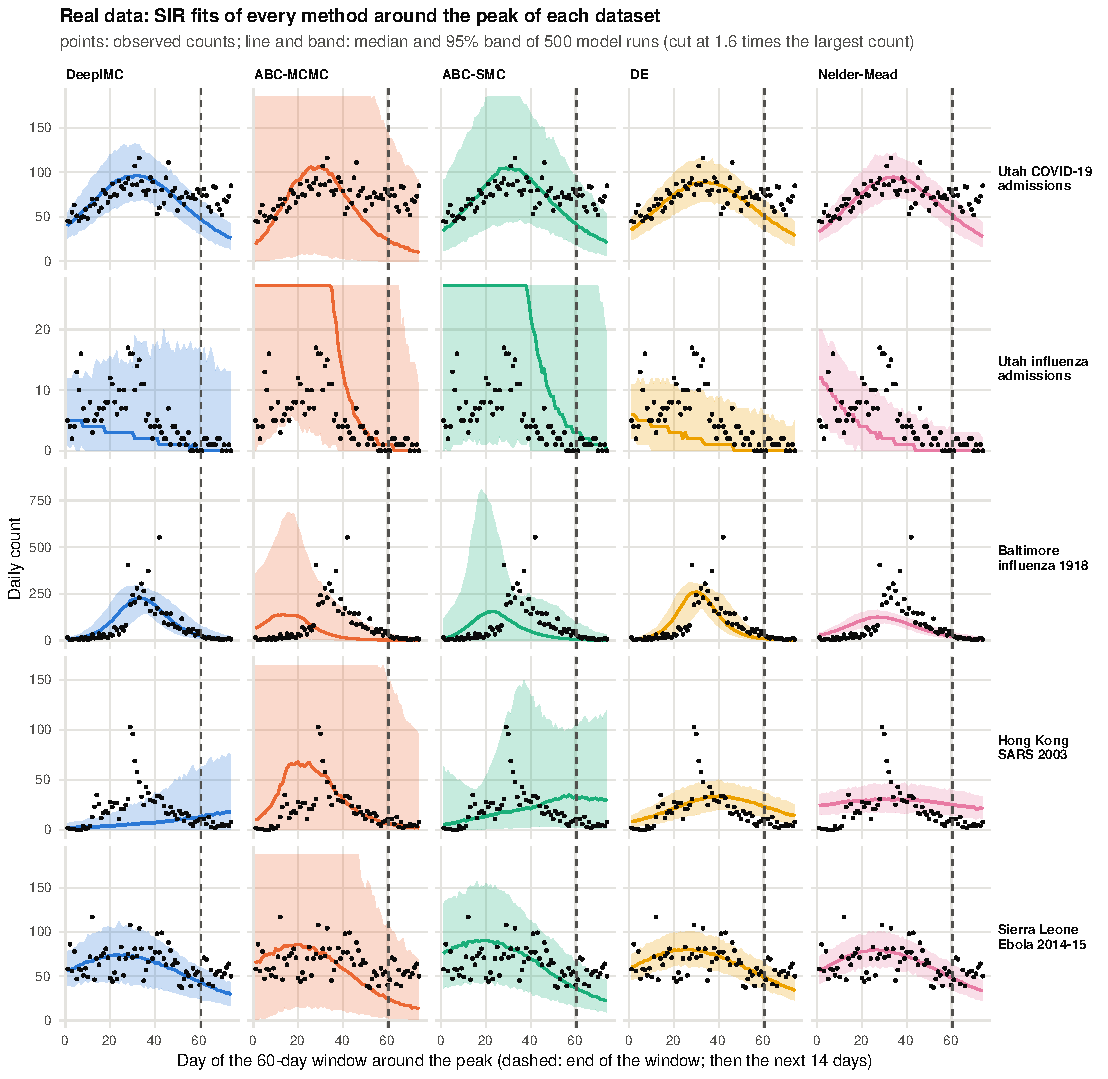
\includegraphics[width=\textwidth]{figures/real_examples_sir.pdf}
\caption{Real data: SIR fits of every method to the 60-day window in the middle of each dataset, as in
Figure~\ref{fig:real-examples}.}
\label{fig:real-examples-sir}
\end{figure}

\section{Supplementary results: predicting with the renewal equation}\label{sec:res-renewal}

Running the agent-based model 500 times for every band is the slowest part of a prediction. The renewal
equation is a deterministic shortcut that gives the model's average curve.

\paragraph{Renewal A.} Started from DeepIMC's estimated state, the renewal equation gave almost the same
curves of new infections as 500 runs of the agent-based model (Table~\ref{tab:renewal}): in the window, a
coverage of 97.5\% against 98.1\% and an MAE of 5.0 against 4.8 for SEIR (96.2\% and 7.8 against 98.9\% and
6.1 for SIR), and the same coverage and MAE over the next 14 days. Its bands for the number currently infectious were narrower than those of the model, because
they contain only Poisson noise around the average and none of the randomness of the epidemic itself, and
covered 86--89\% of the days instead of 98--99\%. On one CPU core, it took 0.18 seconds per SEIR window
instead of 32 seconds for 500 model runs (Table~\ref{tab:timing}).

\paragraph{Renewal B.} Fitting the starting state with the renewal equation did not help. The fitted state was
less accurate than DeepIMC's (2.0 against 1.4 percentage points for SEIR, 2.7 against 2.2 for SIR). The fitted
curve was slightly closer to the observed new infections (MAE 4.4 against 4.8 for SEIR), but from the curve
alone the renewal fit cannot separate exposed from infectious people, and its bands covered the true number of
infectious people on only 39--47\% of the days. Renewal B was also much slower than renewal A, because it fits
the state at 30 values of $R_0$.

\begin{table}[htbp]
\centering
\caption{From DeepIMC's estimates to curves on the simulated test windows: 500 runs of the agent-based
model, or the renewal equation started from DeepIMC's state (A) or from a state fitted by the renewal
equation (B). Starting-state error (percentage points); coverage (\%) of the true curves and MAE of the
median curve; seconds per window during the evaluation, on shared computers (Table~\ref{tab:timing}
compares the times on one dedicated core).}
\label{tab:renewal}
\small
\resizebox{\textwidth}{!}{\begin{tabular}{llrrrrrrrr}
\toprule
 &  & State & \multicolumn{2}{c}{New infections} & \multicolumn{2}{c}{Currently infectious} & \multicolumn{2}{c}{Next 14 days} & Seconds \\
\cmidrule(lr){4-5}\cmidrule(lr){6-7}\cmidrule(lr){8-9}
Model & Curves from & error & Cov. & MAE & Cov. & MAE & Cov. & MAE & per window \\
\midrule
SEIR & model, 500 runs & 1.4 & 98.1 & 4.8 & 98.4 & 17.2 & 98.8 & 1.7 & 16.7 \\
 & renewal A & 1.4 & 97.5 & 5.0 & 88.8 & 18.6 & 98.3 & 1.7 & 0.90 \\
 & renewal B & 2.0 & 96.5 & 4.4 & 38.9 & 21.3 & 97.4 & 1.6 & 68.4 \\
\midrule
SIR & model, 500 runs & 2.2 & 98.9 & 6.1 & 99.0 & 29.7 & 99.1 & 0.7 & 8.1 \\
 & renewal A & 2.2 & 96.2 & 7.8 & 85.5 & 36.7 & 98.3 & 0.7 & 0.49 \\
 & renewal B & 2.7 & 95.3 & 5.3 & 47.2 & 30.8 & 98.0 & 0.6 & 6.02 \\
\bottomrule
\end{tabular}
}
\end{table}

\section{Renewal equation}\label{app:renewal}

With $\beta = R_0\, p_{recov}$ (the daily transmission rate $p_{tran}\, c_{rate}$), $\sigma = 1/\text{incub}$
and $\gamma = p_{recov}$, starting from $S_0$, $E_0$, $I_0$ (the estimated numbers on the first day of the
window), we compute for $t = 1, 2, \dots$
\begin{align*}
\text{new infections}_t &= S_{t-1}\left(1 - e^{-\beta I_{t-1}/N}\right),\\
C_t &= \sigma E_{t-1} \ \text{(SEIR)}, \qquad C_t = \text{new infections}_t \ \text{(SIR)},\\
E_t &= E_{t-1} + \text{new infections}_t - C_t \ \text{(SEIR)},\\
I_t &= I_{t-1} + C_t - \gamma I_{t-1}, \qquad S_t = S_{t-1} - \text{new infections}_t .
\end{align*}
Because the latent and infectious periods are geometric, this recursion equals the renewal equation
(\ref{eq:renewal}) with generation interval $g_k = \sum_{u+s=k} \sigma(1-\sigma)^{u-1}\, \gamma(1-\gamma)^{s-1}$
for SEIR and $g_k = \gamma(1-\gamma)^{k-1}$ for SIR, with the people already exposed or infectious at the
start of the window as its initial condition.

\end{document}
